\documentclass[12pt]{amsart}
%%%%%%%%%%%%%%%%%%%%%%%%%%%%%%%%%%%%%%%%%%%%%%%%%%%%%%%%%%%%%%%%%%%%%%%%%%%%%%%%%%%%%%%%%%%%%%%%%%%%%%%%%%%%%%%%%%%%%%%%%%%%%%%%%%%%%%%%%%%%%%%%%%%%%%%%%%%%%%%%%%%%%%%%%%%%%%%%%%%%%%%%%%%%%%%%%%%%%%%%%%%%%%%%%%%%%%%%%%%%%%%%%%%%%%%%%%%%%%%%%%%%%%%%%%%%   
\usepackage{amssymb}
\usepackage{amsmath}  
\usepackage{amsfonts}
\usepackage{mathrsfs}       
\usepackage{graphicx}
\usepackage{color}   
\usepackage[onehalfspacing]{setspace}
\usepackage{ragged2e}  
\justifying     
\usepackage{caption} 
\usepackage{etex} 
\usepackage{longtable} 
\usepackage{graphicx} 
\usepackage{amsmath}
\usepackage{multirow}
\usepackage{setspace}
\usepackage{footmisc}
\usepackage{amssymb}
\usepackage{amsfonts}
\usepackage[font=bf, justification=centering]{caption}
\usepackage{geometry}
\usepackage{float}
\usepackage{verbatim}
\usepackage{array}
\usepackage{booktabs}
\usepackage{pdflscape}
%\usepackage{xy} 
\usepackage{rotating}
\usepackage[round,authoryear]{natbib}
\usepackage{appendix}
\usepackage{lscape}
\usepackage{subcaption}
\usepackage{graphicx}
\usepackage{amsfonts}
\usepackage{placeins}
\usepackage[utf8]{inputenc}
\usepackage{charter}
\usepackage[colorlinks=true,citecolor=blue,urlcolor=blue,pdfpagemode=UseNone,pdfstartview=FitH]{hyperref}
\usepackage{apptools}
%\usepackage{chngcntr}
\usepackage{multibib}
\usepackage{multirow}
\DeclareUnicodeCharacter{00A0}{'}
%\usepackage[capposition=top]{floatrow}
\newcites{main,supp}{References,References}
%\AtAppendix{\counterwithin{lemma}{section}}
\makeatletter
\def\section{\@startsection{section}{1}
	\z@{1.0\linespacing\@plus\linespacing}{.5\linespacing}{\Large}}

\def\subsection{\@startsection{subsection}{2}
	\z@{.8\linespacing\@plus.7\linespacing}{.7\linespacing}{\large}}

\def\subsubsection{\@startsection{subsubsection}{3}
	\z@{.5\linespacing\@plus.7\linespacing}{-.5em}{\normalfont\bfseries}}
\makeatother                   

\setcounter{MaxMatrixCols}{10}
%TCIDATA{OutputFilter=LATEX.DLL}
%TCIDATA{Version=5.50.0.2953}
%TCIDATA{Codepage=936}
%TCIDATA{<META NAME="SaveForMode" CONTENT="1">}
%TCIDATA{BibliographyScheme=Manual}
%TCIDATA{LastRevised=Friday, May 08, 2015 15:13:41}
%TCIDATA{<META NAME="GraphicsSave" CONTENT="32">}
%TCIDATA{Language=American English}

\numberwithin{equation}{section}

\newtheorem{theorem}{Theorem}[section]
\newtheorem{lemma}{Lemma}[section]
\newtheorem{corollary}{Corollary}[section]
\theoremstyle{definition}
\newtheorem{definition}{Definition}[section]

\theoremstyle{definition}
\newtheorem{assumption}{Assumption}[section]

\theoremstyle{definition}
\newtheorem{example}{Example}[section]

\setlength{\textwidth}{6.5in}
\setlength{\textheight}{9in}
\setlength{\topmargin}{-0.1in}
\setlength{\oddsidemargin}{0in}
\setlength{\evensidemargin}{0in}
\vfuzz4pt
\hfuzz4pt
  

\title{}
\begin{document}
	\vspace*{3ex minus 1ex}
	\begin{center}
		\Large \textsc{Love the Candidate but Hate his Party: \\  The Asymmetric Effects of the Removal of Term Limits on Partisan and Personal Incumbency Returns in Mexico}
		%the Effect of Reelection on Party Dealignment in Mexico} %\\
		%\bigskip  
	\end{center}
	
	
\date{May 28, 2021} 
\vspace*{3ex minus 1ex}
	\begin{center}
		Rafael Ch\\
		
		\textit{New York University}\\
		
	\end{center}
	 
	\thanks{%I thank Pablo Querubin, Cyrus Samii, Hye Young You, Neal Beck, Jacob Shapiro, Juan F. Vargas, Nicholas Haas, Reed Lei, Lucia Motolinia and participants at the Summer Cohort Seminar, Graduate Political Economy Seminar, and Comparative Politics Seminar at NYU, APSA 2020, SPSA 2021, and MPSA 2021 panelists, as well as the members of the Methods and Data Seminar at the University of Wisconsin-Madison for their amazing comments and suggestions. All mistakes are my own.
	\\
	 \\ \textbf{Ch:} Wilf Family Department of Politics, New York University. \\ Email: \url{rafael.ch@nyu.edu}
	 \\ Website: \url{https://wp.nyu.edu/rafaelch/}}
		  
	\begin{abstract}    
	
A large literature has studied the electoral returns to incumbency. However, the estimated incumbency returns in the majority of studies mask an understudied dynamic between parties and their members: both can be hated, loved or differentially liked by their constituency. These scenarios hold different implications on citizens valuation of the electoral system and the existent accountability dynamics. This paper opens up the black box of incumbency by disentangling the personal and partisan incumbency advantages. To do so, I use a difference-in-discontinuity of close elections design in Mexico that exploits the staggered implementation of an electoral reform that introduced reelection for mayors from 2014 to 2022. Term limit elections allow us to identify a partisan advantage while those with candidates up for reelection identify both the partisan and personal incumbency returns. The difference between them identifies the personal from the partisan effect. The main result shows that races up for reelection experienced an incumbency advantage; however, this hides an asymmetry: a personal incumbency \emph{advantage} is found, while parties suffer from an incumbency \emph{disadvantage}. The research design allows to solve several methodological issues of past studies that have tried to disentangle the partisan from the personal effect, primarily rule out potential pretrends of term limit and non-term limit races, as well as concerns on selection coming from the ability and experience of candidates. Overall, the results suggest the personal advantage to be a driving force of incumbency returns, and how  reelection may lead to party dealignment in party-centered systems like Mexico. 
    
	\medskip
	{\noindent \textsc{Key words: Incumbency Advantage, Term Limits, Reelection, Incumbent Resources, Candidates Quality.}}

		%{\noindent \textsc{JEL Classification: %D72, D78, H57, O17.}}
	\end{abstract}
	
	\maketitle
	\pagebreak
   
\section{Introduction}

Over the past decades, an important theoretical and empirical literature has shown that incumbents may enjoy an electoral advantage \citep{ashworth_2012, cox_morgensten_1993, cox_katz_1996, ansolabehere_snyder_2000, ashworth_bdm_2008, ashworth_etal_2019} or suffer from an electoral disadvantage in the next election \citep{klasnja_2015, klasnja_titiunik_2017}. However, whether positive or negative, the electoral returns from incumbency mask an understudied dynamic between the returns associated to parties and those exclusively of candidates. Disentangling both measures is important to understand citizens valuation of the electoral system and the existent accountability dynamics \citep{mayhew_1974, fowler_hall_2014}. For instance, a partisan incumbency advantage might imply that voters believe parties control candidates behaviors, and thus would allow parties to hold a credible threat against renegade candidates. %The implications for a personal advantage are different, however: a personal advantage makes candidates vital for parties electoral success, leading the latter to allow more leeway to the former since retiring or switching parties may hurt parties electoral success. 
However, the implications of a personal incumbency advantage are different from the partisan one. A personal incumbency advantage makes retiring politicians support of new candidates vital for their electoral success, and stepping down or switching parties may hurt their parties in the next election. In this case, parties may allow more leeway to deviate from the party line to their members.\footnote{Likewise, a partisan incumbency disadvantage may imply citizens like partisan balance across time and may create incentives for candidates to differentiate themselves from their parties \citep{klasnja_titiunik_2017}. Contrastingly, a negative personal advantage may lead parties to differentiate themselves from candidates and stop their electoral support or remove the nomination in the next election.} Moreover, if a personal (partisan) effect exists and the partisan (personal) one is negligible it implies voters attribute actions in office to candidates (parties) and not their parties (candidates) or that a party (personal) dealignment might be taking place \citep{cox_katz_1996}.   
   
However, uncovering the partisan and personal incumbency advantage has proved methodologically challenging: every time a candidate is an incumbent so is its party so we cannot uncover the personal from the partisan incumbency advantages. %As a consequence, the personal incumbency advantage is biased (upwardly or downwardly) to changes in the partisan incumbency effects. 
This is true with the most widely used method to estimate the returns to incumbency, the regression discontinuity of close elections design (RDD), that conflates the personal and partisan incumbency advantage, even when the variables are defined in partisan terms (such as likelihood of the party winning or the party vote share) \citep{fowler_hall_2014}. To overcome these obstacles studies have tried to exploit cross-sectional comparisons between term limit and non-term limit races \citep{gelman_king_1990}, expiring and non-expiring careers \citep{fowler_hall_2014}, and changes in redistricting \citep{ansolabehere_snyder_2000, desposato_petrocik_2003, sekhon_titiunik_2012}. However, for identification they have relied on strong assumptions such as no differential pretrends in incumbency returns of term limit and non-term limit races \citep{fowler_hall_2014} or those that experience redistricting or not \citep{ansolabehere_snyder_2004}. %when comparing term-limit and non-term limit elections or expiring vs. non-expiring races  
Moreover,  while studies have used RDDs to rule out potential omitted variable bias coming from the correlation between current and future electoral success including parties reputation and candidates type \citep{klasnja_titiunik_2017}, recent evidence points that differences on the quality of incumbents and challengers -the so called scare-off effect- are still present \citep{eggers_2017}. 

This paper identifies the partisan and personal electoral returns to incumbency and solves the existent methodological difficulties faced by the literature. To do so, I use a difference-in-discontinuity of close elections design that exploits the 2014 Electoral Reform in Mexico that introduced reelection for mayors for the first time. The reform was staggered at the state level which allows us to compare the municipal elections in the not-yet-treated states where term limits exist to those in municipalities where incumbents have the possibility to reelect. Term limit incumbency returns identify the partisan effect as candidates cannot run again for office, while the non-term limit incumbency advantage identifies both the personal and partisan advantages. By differentiating both measures we are able to disentangle the personal from the partisan effect. The difference-in-difference setup allows us to test for parallel trends prior to treatment. Furthermore, by focusing on close elections we rule out potential omitted variables coming from differences in parties and electoral races. Additionally, this paper compares incumbents in their first term only which allows to rule out important endogenous concerns, particularly those arising from selection such as the difference in the ability or experience of incumbents \citep{ferraz_finan_2008, ferraz_finan_2011}. %Lastly, I test for quality differences among incumbents in term limit and non-term limit races, as well as differences between incumbents and challengers. 
 

Results show that the introduction of reelection generated an incumbency disadvantage, i.e., incumbents with the possibility to seek reelection hold a decreasing likelihood to win office in the next election relative to municipalities where candidates are term limited. The same result is found by a decreasing vote share in the next election as a measure for incumbency returns instead of the probability of winning office. However, this incumbency disadvantage masks an asymmetric effect. The incumbency disadvantage is a weighted average of a personal incumbency \emph{advantage} and a partisan incumbency \emph{disadvantage}. This implies incumbency became a personal affair when reelection was introduced in a country with a historically strong party-centered system, Mexico. Results also imply that if candidates retire or switch parties they will hurt the reelection chances of their parties. Not surprisingly, Mexico's 2014 Term Limit Reform introduced a ``parties lock'' where mayors who wish to reelected cannot switch parties.  

To address  methodological concerns, the results are not explained by pre-trends in incumbency advantage or heterogeneous treatment effects between different treated cohorts. Results are robust to various specifications, including varying the bandwidth for close elections and the functional form. Moreover no sorting into treatment or manipulation is found when running the typical McCrary test and testing for no discontinuous jump of other covariates at the winning margin threshold. 

The paper then explores the reasons behind the observed incumbency returns. I do not find evidence of a quality-based incumbency advantage as there are no differences in the quality of term limited and non-term limited incumbents as measured by their education level. I do find evidence, however, of a resource based incumbency advantage where incumbents up for reelection increase the level of municipal revenues, and received an increase in federal and state fiscal transfers relative to term limit incumbents. A personal incumbency advantage may be explained by citizens expecting a higher budget or transfer in the future which they accrue directly to the effort of the incumbent rather than his party. %Interestingly, we also observe a decrease in municipal expenses in social development, infrastructure and public security, and a decrease in the percentage of municipal budget spending (\emph{subejercicios} in Spanish). This could be evidence of how a personal incumbency advantage leads ``incumbents use their office to insulate themselves from electoral pressure'' (\citet{eggers_2017}. 1) and decrease overall spending to focus on particularistic transfers.

The main results of this paper coincide with those of \citet{fowler_hall_2014}, albeit for a different setting. They find that for the U.S. state legislatures the personal advantage is larger than found in previous literature, and that the partisan advantage is zero and possibly negative, as this paper does. This paper is the first one to compare party and personal advantage outside of the US. Moreover, while \citet{fowler_hall_2014} need to assume no pretrends prior to treatment for identification, the difference-in-discontinuity of close elections design allows us to test it and rule it out. 

This paper contributes to the literature on incumbency advantage in party-centered systems. A negative partisan incumbency return and positive personal one affects the way we think about parties-members relationships. Even in the case with strong party systems and a party-lock where candidates cannot run for reelection for other parties, parties cannot credibly threaten to withdraw their support from renegade members. In other words, the introduction of reelection debilitates parties power even in party-centered systems like Mexico generating candidate-centered electoral contests. This goes in line with the partisan dealignment literature, as the one seen in the electorate of the U.S in the post-war era  \citep{cox_katz_1996}, and shows the introduction of reelection to be a possible explanation of such separation between parties and representatives. It also introduced the possibility of new strategic politicians that may work to generate their own incumbency advantage  \citep{mayhew_1974, mckelvey_riezman_1992}.  
 
     
Lastly, this work is closely related to the incumbency disadvantage literature, particularly the work of \citet{klasnja_titiunik_2017}. This paper borrows their measure of party-level incumbency advantage. However, contrary to their setting that studies a weak party system (Brazil) I explore a strong one (Mexico).\footnote{\citet{klasnja_titiunik_2017} classify Mexico as having a weak political party system. Given Mexico's institutional characteristics and historical legacies I believe this to be a misinterpretation.}

The next section delves into the importance of disentangling the personal from the partisan incumbency returns. I then describe the research design, followed by a brief overview of Mexico's 2014 Electoral Reform and data collection. Empirical results are then presented as well as a section with the mechanisms that explain the observed incumbency returns. %I close with a discussion on parties-members relationships when asymmetric personal and partisan incumbency returns are present. 


\section{Personal and Partisan Incumbency Advantage \label{sec:personal_vs_partisan}}

``Incumbency advantage is the additional electoral support a candidate gains due to his or her incumbent status'' (\citet{cox_morgensten_1993}, p. 329). It can be measured as either the difference in the vote share received by the incumbent in the election at $t+1$ from the vote share perceived at election $t$ or the difference in the likelihood of winning office. The literature has found several reasons behind an incumbency advantage from resources, visibility and power gained in office \citep{mayhew_1974, fiorina_1989, king_1991, cox_morgensten_1993}, to differences in the quality of incumbents and challengers \citep{cox_katz_1996, levitt_wolfram_1997, ansolabehere_snyder_2000, eggers_2017}, and the role of information on incumbent's ability and competence to voters \citep{ashworth_bdm_2008, ashworth_etal_2019}. On the other hand, incumbency disadvantage occurs if voters seek to balance power, they dislike parties, or prefer change  \citep{fowler_hall_2014, eggers_2017}, if candidates who replace incumbents or if challengers are of lower quality \citep{eggers_2017}, and/or if parties are weak to control candidates behavior and thus are punished by voters in the following election \citep{klasnja_titiunik_2017}.


Incumbency advantage can be decomposed into two concepts that allow for a better understanding on the relationship between voters, parties and their members: the partisan and the personal incumbency advantages. The partisan incumbency advantage is “the electoral benefit accruing to non-incumbent candidates by virtue of being from the incumbent party” (\citet{fowler_hall_2014}, p. 501). In other words, it speaks to the support parties win in the next election due to their incumbent status. The personal incumbency advantage, however, is a different concept: it is defined as the returns to incumbency that make a candidate better off as an incumbent relative to a candidate for an open seat \citep{fowler_hall_2014}. As such, the personal incumbency advantage has been the typical measure of returns to incumbency in the literature. However, when incumbency returns are estimated the personal advantage is always conflated with the partisan advantage as parties and candidates are incumbents at the same time. 

Consider, for instance, the experiment described by \citet{lee_2008}. He states that in the case of US elections, ``[t]he ideal thought experiment for measuring the incumbency advantage would exogenously change the incumbent party in a district from, for example, Republican to Democrat, while keeping all other factors constant. The corresponding increase in Democrat electoral success in the next election would represent the overall electoral benefit due to being the incumbent party in the district" (p. 683). To proxy for this thought experiment, \citet{lee_2008} runs an RDD of close elections comparing the returns to incumbency in the next election $t+1$ for incumbents who barely win to those that barely lost at the election in $t$. However, the resulting incumbency returns provide an entangled average effect of both the personal and partisan incumbency return. Moreover, experiments such as this tend to interpret the results as accruing solely to incumbents rather than their parties, and do not consider voters may value differentially parties and their representatives. 

Substantively, these two concepts provide different interpretations of the electoral system. Overall there are six possibilities. First, we can observe a  partisan and personal incumbency \emph{advantage}. In this case, positive incumbency returns increase the concern that incumbents may insulate themselves from electoral threats, and debilitate their accountability to constituents \citep{ashworth_etal_2019, cox_katz_2002}. Parties might not have incentives to monitor or exercise control over their members given their electoral isolation as well as the potential negative consequences of standing against incumbents with high personal electoral returns from office. Overall, a personal and partisan incumbency advantage may signal that voters accrue actions of candidates to both parties and representatives, and may lead parties and candidates to isolate from the electoral connection created by reelection \citep{mayhew_1974}. 

 In a second scenario, we can observe both a partisan and personal incumbency \emph{disadvantages}. A negative partisan incumbency may show constituents prefer partisan balance \citep{folke_snyder_2012}, believe the ``grass-is-greener'' with other parties \citep{bhatia_turan_2013}, dislike institutions relative to their members \citep{parker_davidson_1979}, or have suffered from institutional changes such as redistricting that decreases electoral support of incumbents \citep{ansolabehere_snyder_2000, desposato_petrocik_2003}, for example. A negative personal incumbency might signal voters see incumbent politicians as too corrupt and prefer new candidates to hold office in the next turn. In this setting, parties choice might be to nominate new candidates to contend for office despite incumbents holding the possibility to reelect. Incumbents up for reelection may choose to switch parties or run for other political positions at the state or federal level in which case they may be very diligent in following the party line. 
  
 Third, we can observe an asymmetry where a personal incumbency \emph{advantage} might coincide with a partisan incumbency \emph{disadvantage}. Parties no longer hold a credible threat to punish renegade incumbents. Moreover, a retirement slump might lead parties to lose votes when the incumbent retires \citep{alford_brady_1989} or in the presence of term limits \citep{ansolabehere_snyder_2004}. Candidates may also hold incentives to differentiate themselves from their parties through various personalistic strategies as voters may attribute the actions of candidates only to them and not their parties. A positive personal incumbency might also imply voters transfer their support to whomever the current incumbent wishes to endorse if they are retiring. A personal incumbency advantage might also signal a sophomore surge when a new representative will garner more votes when running for his first reelection than when she was a challenger \citep{erikson_1971, alford_brady_1989}. 
  
 
 Fourth, an asymmetry with a personal incumbency \emph{disadvantage} might coexist with a partisan incumbency \emph{advantage}. In this case, citizens might see representatives as lame ducks in office and attribute their actions to their parties. In this setting we may also have that retiring incumbents are not invited to support new candidates from their party as this may damage their electoral success in the coming election. More importantly, this scenario makes elections party-centered rather than candidate-centered, with parties holding a credible threat to withdraw their support or nomination for dissident members since new candidates will benefit from the positive partisan electoral return for the next election.  

The two additional scenarios are for either partisan or personal incumbency returns to be negligible. When the personal incumbency is not different from zero, it may imply that actions of incumbents do not affect the parties return from incumbency if they choose to step aside by switching parties or retiring. On the contrary, a negligible partisan incumbency return makes the branding and attributes of parties not as important for voters even if they rely on partisan labels to define their vote. Moreover, voters in this setting might see the actions of incumbents as separate from their parties \citep{fowler_hall_2014}. 

A negligible or negative partisan incumbency return and a personal incumbency advantage is strongly tied to the large literature on partisan dealignment. As \citet{beck_1985} notes, an electorate that appears to be highly partisan may be just a facade if ``partisanship is merely an expression of momentary vote choice'' (p. 233). This dealignment trend has been identified in the US since the 1953 due to generational changes, as well as the weakening of group bases of party support and increase electoral competition \citep{beck_1977, norpoth_rusk_1982}, in Britain since 1970 due to retrospective voting \citep{alt_1977}, the Netherlands since the late 1960s due to vote switching and the decline in political cohesion of groups \citep{irwin_dittrich} and Denmark, Norway and Sweden were class voting declined since the 1970s \citep{borre_1995}. In Mexico -the study case at hand in this paper-, winning margins have substantively declined since the move to democracy in 2000, while party bases have constantly migrated from one party to another, and from one political leader to another. Besides the case of the US, however, partisanship has been linked too closely to candidate vote choice to assess whether dealignment ocurrs.  However, the existence of a strong personal incumbency advantage relative to a negligible or negative partisan one, for example, may portray a dealignment of citizens from mass politics and into more personalistic electoral contests. 
   
As described thus far, evaluating an electoral system requires the identification of the personal and partisan incumbency returns. Limiting to the former provides and incomplete picture of the dynamics between voters, parties and their members. 

Take for example the case of Mexico. Prior to the introduction of the 2014 Term Limit Reform, Mexico had a party-level incumbency disadvantage. With term limits in place, the likelihood of incumbent parties to win office in the next election where negative and close to -28\% according to \citet{klasnja_titiunik_2017}, who take into account all mayoral elections from 1997 to 2009. Appendix \ref{appendix:rdd} runs a similar experiment with an RDD with close elections and optimal bandwidths following \citet{calonicoetal_2014} but considering all mayoral races from 1989 to 2018. Since this time period covers races before and after the 2014 Electoral Reform, i.e., with and without term limits, I ran two separate RDDs. I find an incumbency disadvantage of -11\% significant to the 1\% level, using both a linear and quadratic polynomial. An incumbency disadvantage is also found using vote share of -4\% significant to the 1\% level using a linear and quadratic polynomial as well. Contrastingly, for elections that removed term limits and introduced reelection for mayors we observe a positive but not significant effect on incumbency returns, using both the probability of victory or the winning margin in the next election. In other words, it seems reelection erased the negative returns to parties in Mexico. However, these incumbency returns estimates do not allow us to assess whether incumbency became a personal matter when reelection was introduced or remained mainly a partisan one. In other words, we are unable to securely state that Mexico moved from a party to a candidate centered system due to the introduction of reelection and the strengthening of voter accountability, and what this implies in terms of of voters, parties, and representatives dynamics.

 Moreover, these estimates may be biased in three ways. First, by comparing term limit and non-term limit elections we need to assume there are parallel trends which might not be the case and an RDD does not allow us to test this assumption. Second, there might exist heterogeneous treatment effects across different treatment cohorts since the 2014 Electoral Reform was implemented in a staggered way at the state level. Lastly, as \citet{eggers_2017} notes even when comparing close elections in a regression discontinuity design, a potential difference in the quality of incumbents and challengers may still exist. The next section addresses these methodological issues by describing the research design used in the paper.  

  
\section{Research Design to Disentangle the Personal from the Partisan Incumbency Advantage \label{sec:design}}

The typical methodological tool to study incumbency returns is the regression discontinuity design (RDD) \citep{thistlethwaite_etal_1960, imbens_lemieux_2008, lee_2008}. Since election results are not exogenous, we move to a local environment where we compare very close elections. Presumably, by comparing incumbents that barely won to those that barely lost we have identical candidates and parties on each side of the cutoff \citep{lee_2008, boas_hidalgo_2011, broockman_2009, butler_2009, dalbo_etal_2009, querubin_snyder_2013, titiunik_2012, klasnja_titiunik_2017}. However, recent evidence shows that even with RDDs of close elections barely winners and losers might differ in terms of quality \citep{eggers_2017, caughey_sekhon_2011, grimmer_etal_2012}. Problems include incumbents being better than challengers or a potential scare-off effect. 

RDDs, moreover, cannot disentangle the personal and party incumbency advantages. As \citet{erikson_titiunik_2015} show, the RDD coefficient is defined as 2*Partisan Advantage + 2*Pr(Winner Runs Again)*Personal Advantage. This makes the partisan and personal advantage unidentified. A possibility to disentangle them is to compare two different regression discontinuity models, one for elections with term limits where no candidate can remain in office more than the appointed term, and one for elections with the possibility to reelect at least one term. \citet{fowler_hall_2014} show that the difference between these two models yields the personal incumbency advantage, since the term limit one captures the partisan effect and the non-term limited model the partisan and personal effect. For this difference to yield identified personal and partisan effects, however, we need to rely on three identification assumptions. First, as with any RDD of close elections, that potential outcomes are continuous at the forcing variable threshold, i.e. the electoral vote share. This implies that the current and next election support the same parties in contestation. The second assumption states that the average personal and partisan incumbency advantages in a given election do not vary differently across time for those with and without term limits. This assumption is the typical parallel trend assumption in difference-in-difference (DiD) designs. As with DiDs, the parallel trend assumption does not imply that term limit and non-term limit elections are the same across covariates, but that the vary similarly across time prior to treatment. However, in the case of term limit and non-term limit races it is a very strong assumption. \citet{fowler_hall_2014} rely on various tests to assess this assumption including comparing legislative elections in states with term limits and without, the latter being a placebo. However, state legislatures vary in different characteristics across time such as the quality of challengers and potential scare-off effects \citep{rogers_2014}. The third identification assumption is that there is no change in the quality of incumbents when an incumbent retires as is replaced by a new candidate. 


Other papers have tried to disentangle the personal from the partisan incumbency advantage. By definition, a personal incumbency advantage comes from comparing the electoral returns of an incumbent up for reelection to the same seat -in the same election and locality at the same time- but with term limits. This makes the open seat a counterfactual scenario. A similar experiment in mind is that of \citet{gelman_king_1990} that compares two scenarios, one where the incumbent legislator runs, and another when it retires, and both accrue to the same party. Holding the party constant allows to tease the party incumbency advantage. The concern is that races where incumbents retire might not have the same trends to those where they do not. Another experiment has exploited redistricting, where the personal incumbency return comes from comparing  new voters who are first experiencing and incumbent are compared to old voters who already know the incumbent \citep{sekhon_titiunik_2012}. The problem, however, is that even conditional on covariates old and new voters may differ introducing potential bias as noted by a large gerrymandering literature. 

To overcome these empirical challenges and relax the  assumptions to identify the personal and partisan incumbency advantages, I leverage a difference-in-discontinuity design that exploits the staggered rollout of an Electoral Reform in Mexico in 2014 that removed term limits and compares only mayoral close elections. Term limited incumbents are forced to retire but not their parties allowing to identify a partisan incumbency advantage. Meanwhile incumbents are for reelection identify the party and personal incumbency advantage. The difference between the average probability of winning in the next election $t+1$ (or vote shares) of those competing in term limited elections relative to non-term limited ones in the election at $t$ would provide an unbiased estimate of the personal (A) and partisan incumbency advantage (B). Meanwhile, the effect of term-limit races would provided an unbiased estimate of the partisan incumbency advantage (B). By differentiating these two quantities (A+B-B=A) we can obtain an unbiased estimate of the personal incumbency advantage. The difference-in-discontinuity of close elections design allows us to test for parallel trends instead of assuming such trends exist prior to treatment as other studies do.

Importantly, the aforementioned quantities needs to be divided by 2 and take into account the probability of an incumbent running again for office as some may retire. As described by \citet{fowler_hall_2014} making a reference to the findings of \citet{erikson_titiunik_2015} ``the partisan incumbency advantage is doubled because the winning party has both the benefit of being the incumbent party and the benefit of the other party not having this advantage. Similarly, if we knew that the winner of the first election would always run for re-election, then the RD estimate would also include two times the personal incumbency advantage. However, the incumbent does not always seek re-election, so we must multiply this term by the probability that the winner of a close election seeks re-election'' (p. 512). 

Furthermore, in this paper instead of assuming that the quality of an incumbent that retires is similar to that of the new candidate, I test whether we observe quality differences in incumbents that barely won in term limited and non-term limited electoral races. Also, by comparing first term to second term incumbents in both term limit and non-term limit elections I test whether a potential scare-off effect exists, i.e. the tendency of incumbents to deter strong challengers. Presumably this is a good way to test the scare-off effect since challengers would be more concerned of facing an incumbent in its second term given the increase in experience rather than those in their first term. 

Lastly, the research design only compares first term mayors in term limit and non-term limit races. This comparison erases the concern on differences between experience or ability between candidates up for reelection or bounded by term limits \citep{ferraz_finan_2008, ferraz_finan_2011}. For clarity on the treatment, the next subsection provides a description of the 2014 Term Limit Reform in Mexico.  

\subsection{Mexico's 2014 Term Limi Reform}

In Mexico in 1933, the Partido Nacional Revolucionario (PNR, the former PRI) imposed a ban on reelection making all presidential, gubernatorial, legislative and mayoral elections term limited. The motivations behind this constitutional amendment was to control self-motivated politicians to deviate from the party line in any of the multi-level party structure. The famous phrase in Mexican politics ``if you move you don't appear in the photo'' (\emph{si te mueves no apareces en la foto}) which implies that if you deviate from the party line you will be left aside, shows the spirit of the PNR and later the PRI to weaken  local party bosses and allow the party to control political careers at the federal, state and local level by limiting reelection \citep{weldon_2003}. 

Eighty years later in 2013, the new Peña Nieto administration pushed an aggressive set of reforms to privatize the energy sector and modify the existent fiscal institutions in the country. To increase the probability of success, the PRI with the PAN and PRD, the three main political parties at the time, lead the construction of the Mexican Pact Accord, a series of roundtables intended to negotiate the energy sector reform along a set of structural reforms that had fail to pass through congress due to political gridlocks. By the end of May 2013, a roundtable to discuss an electoral reform was installed. Specifically, commitment 94 of the Pact Accord introduced reelection for discussion. While the Electoral Reform was not under PRI's set of desired reforms, the opposition utilize it as a bargaining chip to approve those pursued by the PRI \citep{zamitiz_2017}. However, due to lack of consensus, the Mexican Pact Accord did not submit an electoral reform proposal to Congress and left the bargaining process to the Senate. Two months later, on July 24, 2013, PAN and PRD pushed a political-electoral reform with 36 law changes that included  the creation of a National Electoral Institute (INE for its acronym in Spanish) that would be in charge of federal, state and local elections, and reelection for federal and local legislators, as well as mayors. Given state-level opposition to the reform, Senate leaders from the PAN and PRD chose to approve the electoral reform in December 2, 2013, before the energy reform, and thus increased their political leverage over the PRI. By January 2014, PAN and PRD threatened to back the energy reform  if the PRI did not push local state legislatures from approving the electoral reform which at the time where blocking the reform given pressure from various PRI governors.\footnote{The Mexican Constitution establishes that the majority of state legislatures need to approve constitutional reforms for reforms to be valid.} The political gridlock led former President Peña Nieto to ``exhort" local legislators to approve the electoral reform. On January 31, 2014, the reform was promulgated by the President and contained three main changes: (1) the creation of the INE; (2) removal of term limits of mayors for up to 2 terms;\footnote{The reform also introduced reelection for local and federal legislators who are allowed to reelected up to 4 consecutive terms.} and (3) the introduction of a ``parties-lock"	where mayors or legislators who wish to reelected could not switch parties.\footnote{For more details on the political background of the 2014 Electoral Reform please see Appendix A in \citet{ch_2021}.}

The reform granted discretion to state legislatures to define the number of terms mayors could reelect as well as the reelection implementation date. All states approved up to 2 consecutive reelection terms for mayors except for the states of Nayarit, Hidalgo, Tlaxcala and Veracruz who did not allowed consecutive reelection. 
  
In regards to the implementation date, the Electoral Reform established that it would not affect any of the 2014 elections. Figure \ref{fig:treatment_status} describes the implementation period or treatment status of each of Mexico's 32 states.\footnote{Mexican states share the same administrative level as US states.} This figures allows to visualize the staggered rollout of the term limit removal. We have five timing groups. Four states never receive treatment during this time period (Hidalgo, Nayarit, Tlaxcala and Veracruz), while the rest commence treatment in different years from 2015 to 2019. Evidence suggests that the differences in timing is a function of the staggered calendar of gubernatorial elections. As noted by \citet{motolinia_2020}, at the moment the reform was approved some governors were starting their terms while others were ending them. Those ending their terms had greater incentives to introduce reelection early on given that they could still apply political influence after leaving office by choosing people of their liking. In other words, governors influence in candidate selection of mayors seems to explain most of the variation in the staggered calendar of the implementation of the reform. For causal identification, it is important in empirical specifications to control for governors political power. 
   
\begin{figure}[h]   
\centering 
\caption{Mexican States Electoral Reform Treatment Status}
\label{fig:treatment_status}
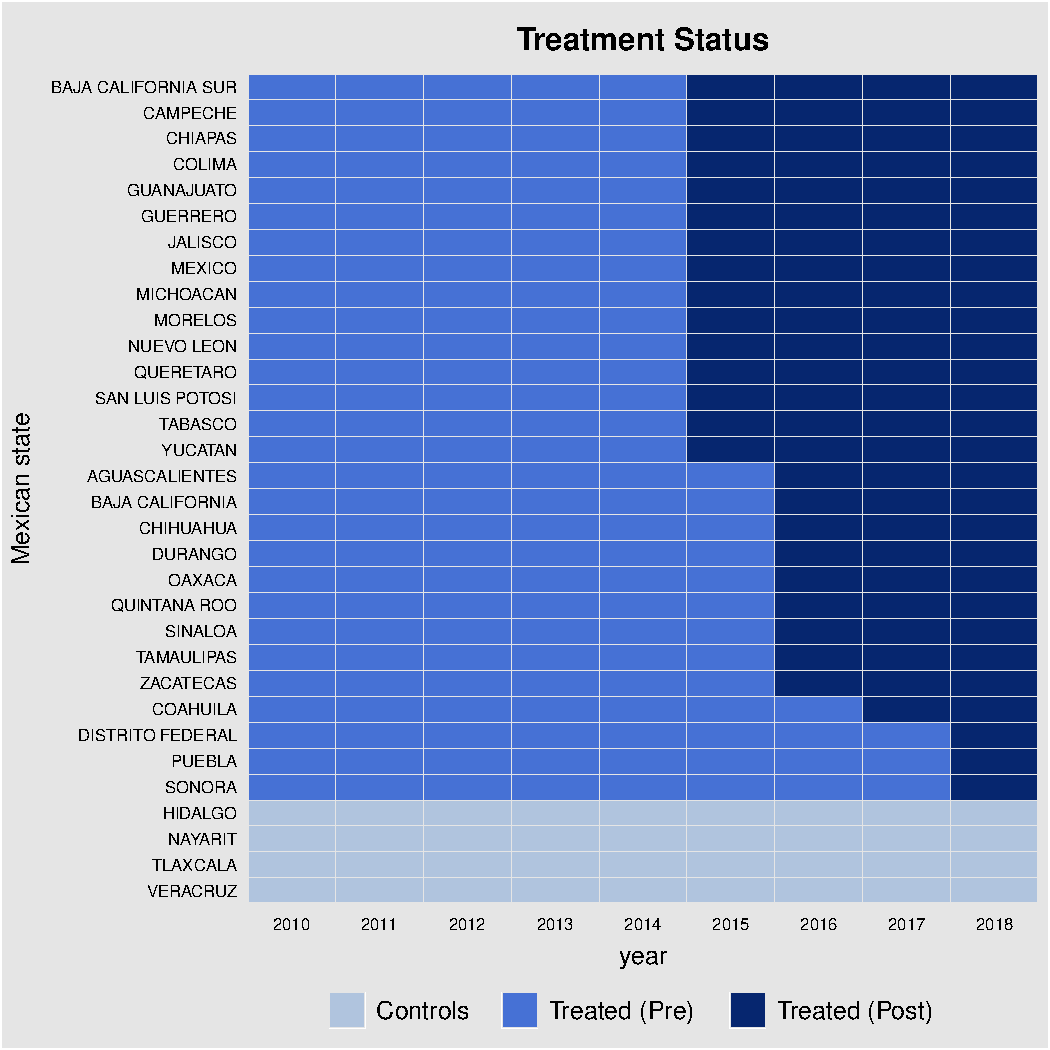
\includegraphics[width=0.75\textwidth]{../Figures_incumbency/reform_treatmentstatus.pdf}     
\captionsetup{justification=centering} 
\end{figure}         

\subsection{Empirical Specification}  

I estimate  a difference-in-discontinuity design with close elections that exploits the staggered implementation of the 2014 Electoral Reform  and state-level variation.
      
Following \citet{grembi_2016} and \citet{gelman_imbens2014}, I fit a local linear regression for municipalities within an \citet{calonicoetal_2014} optimal bandwidth distance $h$ to the cutoff (=0), using as forcing variable the winning margin of executive local elections.\footnote{A rectangular kernel would give the same results as taking $E[Y]$ at a given bin on the distance to the cutting threshold. Other types of kernels, such as a triangular kernel, gives more weight to observations closer to the cutoff. I choose the latter for all estimations presented while estimations using a rectangular kernel are available upon request. Results are almost unchanged using the latter rather than the former.} In other words, I compare only municipalities in close elections and thus restrict the sample to those within a certain distance $h$ to the threshold, i.e. $D_{mt} \in [D_b-h, D_b+h]$ for municipality $m$ in time period $t$. By comparing municipalities where a party barely wins an election to municipalities where a party barely loses, the design allows to isolate the causal effect of winning office from the spurious correlation between current and future electoral success.\footnote{For example, potential correlation that could arise, noted by \citet{klasnja_titiunik_2017}, is that parties with good reputation or strong candidates are more likely to succeed in an electoral contest.} 

Furthermore, the difference-in-difference setup allows to tease out any time-variant and time variant confounding variation as long as parallel trends and no anticipatory behavior from municipalities (states) holds. For this I rely on \citet{abraham_sun_2020} cohort weighted event-study design that accounts for potential cohort treatment heterogeneity. I saturate the time and unit fixed effects structure so that treated units do not enter the test window as control units. Specifically, I replace the binary indicator variable for the start of the 2014 Electoral Reform in Mexico with a series of lead/lag indicators $\gamma_k$ for being ``k" years away from treatment. I focus on the window from 7 years prior to treatment to the year in which the reform took place i.e. for $k \in \{-7,0\} $ which correspond to the time period of 2011 to 2018, with 2015 the first year of Term Limit Reform implementation. Given that municipal elections occur every three years at maximum, and the reform was enacted in 2014 and all municipalities in the study period had only one election, there are no leads. Moreover, there are no mayoral elections in $t-1$ and $t-2$. Thus $k$ relative time periods run from  $k \in\{-7,-6,-5,-4,-3,0\}$. Following \citet{abraham_sun_2020} I exclude the indicator prior to treatment  $\gamma_{-3}$ to avoid collinearity and for comparison: estimated coefficients are interpreted as the difference relative to $t-3$, i.e. the last election. As suggested   \citet{abraham_sun_2020}, I also exclude the last time period $k=-7$ due to collinearity.

The specification of the difference-in-discontinuity in close elections design is the following:

\begin{equation}
\begin{split}
\label{eq:abraham}
y_{mt}=\mu_m + \mu_t + \sum^5_{e=1} \sum^0_{k=-6, \neq {-7,-3}} \gamma_{e,k}(1\{E_i=e\} \cdot R^k_{m,t}) + \sum^5_{e=1} \sum^0_{k=-6, \neq {-7,-3}}  \Theta'X_{it} (\mathbbm{1}(E_i=e)\cdot R^k_{m,t})  \\
+ f_{(.)}(margin)_{mt} + \sum^5_{e=1} \sum^0_{k=-6, \neq {-7,-3}} \nu_{e,k}(1\{E_i=e\} \cdot R^k_{m,t} \cdot  f_{(.)}(margin)_{mt} )+ \epsilon_{mt}
\end{split}
\end{equation}   
  
where $y_{mt}$ is the outcome of the probability of winning office or the winning margin in the next election $t+1$. $E_i$ are cohort-specific indicators if a Mexican state removed term limits in a given year.\footnote{As noted in Figure \ref{fig:treatment_status}, there are five treatment cohorts including the never treated. The never-treated cohort is made up of the municipalities in the states of Hidalgo, Nayarit, Tlaxcala and Veracruz.} $R^k_{m,t}\in \{0,1\}$  is the Term Limit Reform treatment status indicator at period $k$ relative to treatment, for municipality $m$ at calendar time $t$.\footnote{$t=e+k$.} $X_{s(m)t}$ is a matrix of state $s$ (municipal $m$) level covariates interacted with the set of cohort-specific fixed effects including pre-treatment governor's winning margin, party alignment with the governor, party alignment with the President, and logged population.  The year indicators by treatment cohort  $\gamma_{e,k}$ are the difference-in-difference (DiD) estimators for the Cohort Average Treatment Effects (CATTs). Conditional on municipal and period fixed effects, as well covariates, these CATTs represent the annual difference in the probability of winning (or the winning margin) in the next election $t+1$ for mayors without term limits to those with term limits, $k$ years before and after treatment. $f_{(.)}(margin)_{mt}$ is the RD polynomial on winning margin for municipal election $m$ at calendar time $t$, having $f_{(.)}$ take various polynomial approximations from quadratic to quartic. $\sum^5_{e=1} \sum^{0}_{k=-6, \neq {-7,-3}} \nu_{e,k}(1\{E_i=e\} \cdot R^k_{m,t} \cdot  f_{(.)}(margin)_{mt}  $ is the RD polynomial interacting the $E_i$ cohort-specific indicators and the electoral reform treatment indicator. 

I then take the linear combination of the CATTs for each relative time period $k$, weighting each cohort by its relative share of the sample, to construct the interaction weighted (IW) estimator of \citet{abraham_sun_2020}:   

\begin{equation}
\hat{\nu}_g=\frac{1}{|g|}\sum_{k \in g}\sum_e \hat{\gamma_{e,k}} \hat{Pr}\{E_i=e | E_i \in [-k, T-k]\}	
\end{equation}
  
where $\hat{\gamma_{e,k}}$ is returned from equation \ref{eq:abraham} and $\hat{Pr}\{E_i=e | E_i \in [-k, T-k]\}$  are the estimated weights equal to the share of each cohort in the relevant time period, normalized by the size of  $g$, with $g$ the universe of the $k$ periods relative to treatment. Since I estimate a IW estimator per year $|g|=1$. Lastly, to estimate the average treatment effect for $t=0$, I run the linear average of weighted coefficients across the CATTs of this time period relative to treatment.  Standard errors are clustered at the state level as that is the level of treatment of the Electoral Reform in Mexico. 

\subsection{Data}

To measure incumbency advantage, I construct an indicator that takes the value of 1 if the party won office in the next election and was an incumbent two elections before, 0 otherwise. This analysis identifies the party that wins in the next election and studies the effect of this party barely winning (or losing) in the present election on outcomes at the next election following \citet{klasnja_titiunik_2017}. This measure requires at least three rounds of elections, and thus I consider all municipal level elections since 2011 to 2018.\footnote{Municipal electoral calendars vary by state. However, almost all municipalities have three year terms with the exception of some municipalities with non-aligned electoral calendars with State-level ones, or other political circumstances.} A second measure uses vote share instead of the probability of winning office. Different from the Brazilian case studied by \citet{klasnja_titiunik_2017} where parties do not contest in every election and thus need to adjust estimates unconditional on parties running,\footnote{\citet{klasnja_titiunik_2017} called this outcome ``unconditional victor on running" and measures if a party won at $t+1$ regardless of whether they had a candidate at that time period or not.} in Mexico the three main parties in this time period (PRI, PAN and PRD) always run in elections they have already participated in the past and hold national representation. Thus, there is no bias to be concerned of related to a party's decision to run at $t+1$ given anticipation of their performance at that same time period.  

To measure incumbent quality, I web-scraped professional titles and other characteristics for all municipal mayors in Mexico from 2010 to 2019 from the National Information Municipal System (SNIM for its abbreviation in Spanish). This novel database allows me to test for quality-based incumbency advantages.

I use several measures to proxy for the resources and effort placed by incumbents once in office. I use the National Institute of Statistics and Geography (INEGI for its acronym in Spanish) municipal level data on revenues and expenses from 2010 to 2018. I use data on total municipal revenues, as well as its subcomponents, specifically those coming from taxes, including property and estate taxes, as well as those from production, consumption and transaction taxes. These variables were deflated and are expressed in million pesos. The data is further described in Section \ref{sec:mechanisms} while Appendix Table \ref{tab:descriptive} presents descriptive statistics.

%The last piece of information used in this paper are municipal expenses on different topics including social development, infrastructure, wages to bureaucrats and public security. The allow to test incumbents' interest in public good provision. This data also comes from INEGI and covers the time period from 2010 to 2018. These variables are deflated and expressed in million pesos. 

\section{Main Results \label{sec:results}}

Figure \ref{fig:main} presents the IW estimators on the effect of reelection on incumbency returns. The first point estimate from top to bottom shows that mayors up for reelection experience an incumbency disadvantage of -7.23\% in the probability of winning office in the next election using a linear polynomial specification. This result is not significant however, while an incumbency disadvantage of -13.25\% significant to the 5\% level is found for the quadratic polynomial specification. Appendix Table \ref{tab:incumbency_wpolynomials} shows the incumbency disadvantage is also found when using winning margin in the next election as an outcome instead of the probability of winning, with a decrease of -1.75\% significant to the 5\% level with a linear polynomial, and -1.26\% significant to the 10\% level with a quadratic polynomial. These results suggest mayors up for reelection face an incumbency disadvantage relative to mayors in term limit races.   

However, as noted in Section \ref{sec:personal_vs_partisan}, this incumbency disadvantage masks an asymmetric effect. In Figure \ref{fig:main} we observe that the incumbency disadvantage is a weighted effect of a personal incumbency \emph{advantage} of 24.7 percentage points significant to the 1\% level and a partisan incumbency \emph{disadvantage} of -31.9 percentage points significant to the 5\% level using a linear polynomial. Similar results are found with a quadratic specification.\footnote{From here on, all estimates are divided by 2 times the probability of the incumbent running for office again following \citet{erikson_titiunik_2015}.}$^,$\footnote{Appendix Figure \ref{fig:personal_vs_partisan_margin} shows similar asymmetric effects using winning margin in the next election as outcome to proxy for incumbency advantage. In this case there are positive but not significant personal incumbency returns and negative partisan incumbency returns significant to the 5\% level using a linear specification. Using a quadratic specification we find more noisy results.} While these incumbency returns might seem large, these values coincide with large incumbency returns observed in other Latin American countries. The incumbency disadvantage in Brazil is -15\%, while in Colombia and Peru is -20\% and -19\%, respectively, according to \citet{klasnja_titiunik_2017}, for example. Moreover the partisan incumbency disadvantage identified by \citet{klasnja_titiunik_2017} for term limit races in Mexico from 1997 to 2009 of -28 percentage points coincides with the partisan incumbency disadvantage of -31\% described above. 
   
As noted in Section \ref{sec:personal_vs_partisan}, prior to the 2014 Reelection Reform, Mexico's mayoral elections showed a partisan incumbency disadvantage. Once reelection is introduced a decrease in the incumbency disadvantage is observed and in the linear specification of Figure \ref{fig:main} it is statistically not different from zero. This decay in the incumbency disadvantage with the removal of term limits is similar to the finding by \citet{klasnja_titiunik_2017} when comparing the incumbency returns from countries with term limits -mainly Brazil, Mexico, and Colombia-  to those with indefinite reelection -Peru, Chile and Costa Rica: while the former show an average incumbency disadvantage of -19\% (significant to the 1\% level) the latter show an incumbency disadvantage of -2\% (non-significant). In the case of \citet{klasnja_titiunik_2017} they believe incumbency disadvantage is explained by voters blaming weak parties from not being able to sanction their members from undesirable behavior in office, specially when they are term limited and there is no need to be responsive for voters. Reelection in this setting strengthens the accountability between voters and representatives which should decrease the responsibility put on parties to control their members decreasing the incumbency disadvantage. The asymmetry found in Figure \ref{fig:main} offers a closely related logic: reelection creates an ``electoral connection'' between voters and incumbents \citep{mayhew_1974}; as a result a personal incumbency advantage is created signaling that voters believe incumbents and not their parties are responsible for policy actions. %Without reelection, as is the case with term limits, politicians do not hold any benefit from impressing the voter and thus will not be responsive to them \citep{ashworth_2012}.
 In other words, a personal incumbency advantage is the main driver in the decrease in incumbency disadvantage in Mexico, and plausibly other countries too.

Moreover, this result speaks to a potential party dealignment in Mexican politics after the introduction of reelection. Not only has the country experienced a decrease in winning margins and various changes in party bases in the last two decades, but citizens at the municipal level are associating policy actions to representatives rather than their parties. 
       
 \begin{figure}[h]   
\centering    
 \caption{Effect of Term Limit Reform on Partisan and Personal Incumbency Advantage \\ -difference-in-discontinuity of close elections design-}
 \label{fig:main}
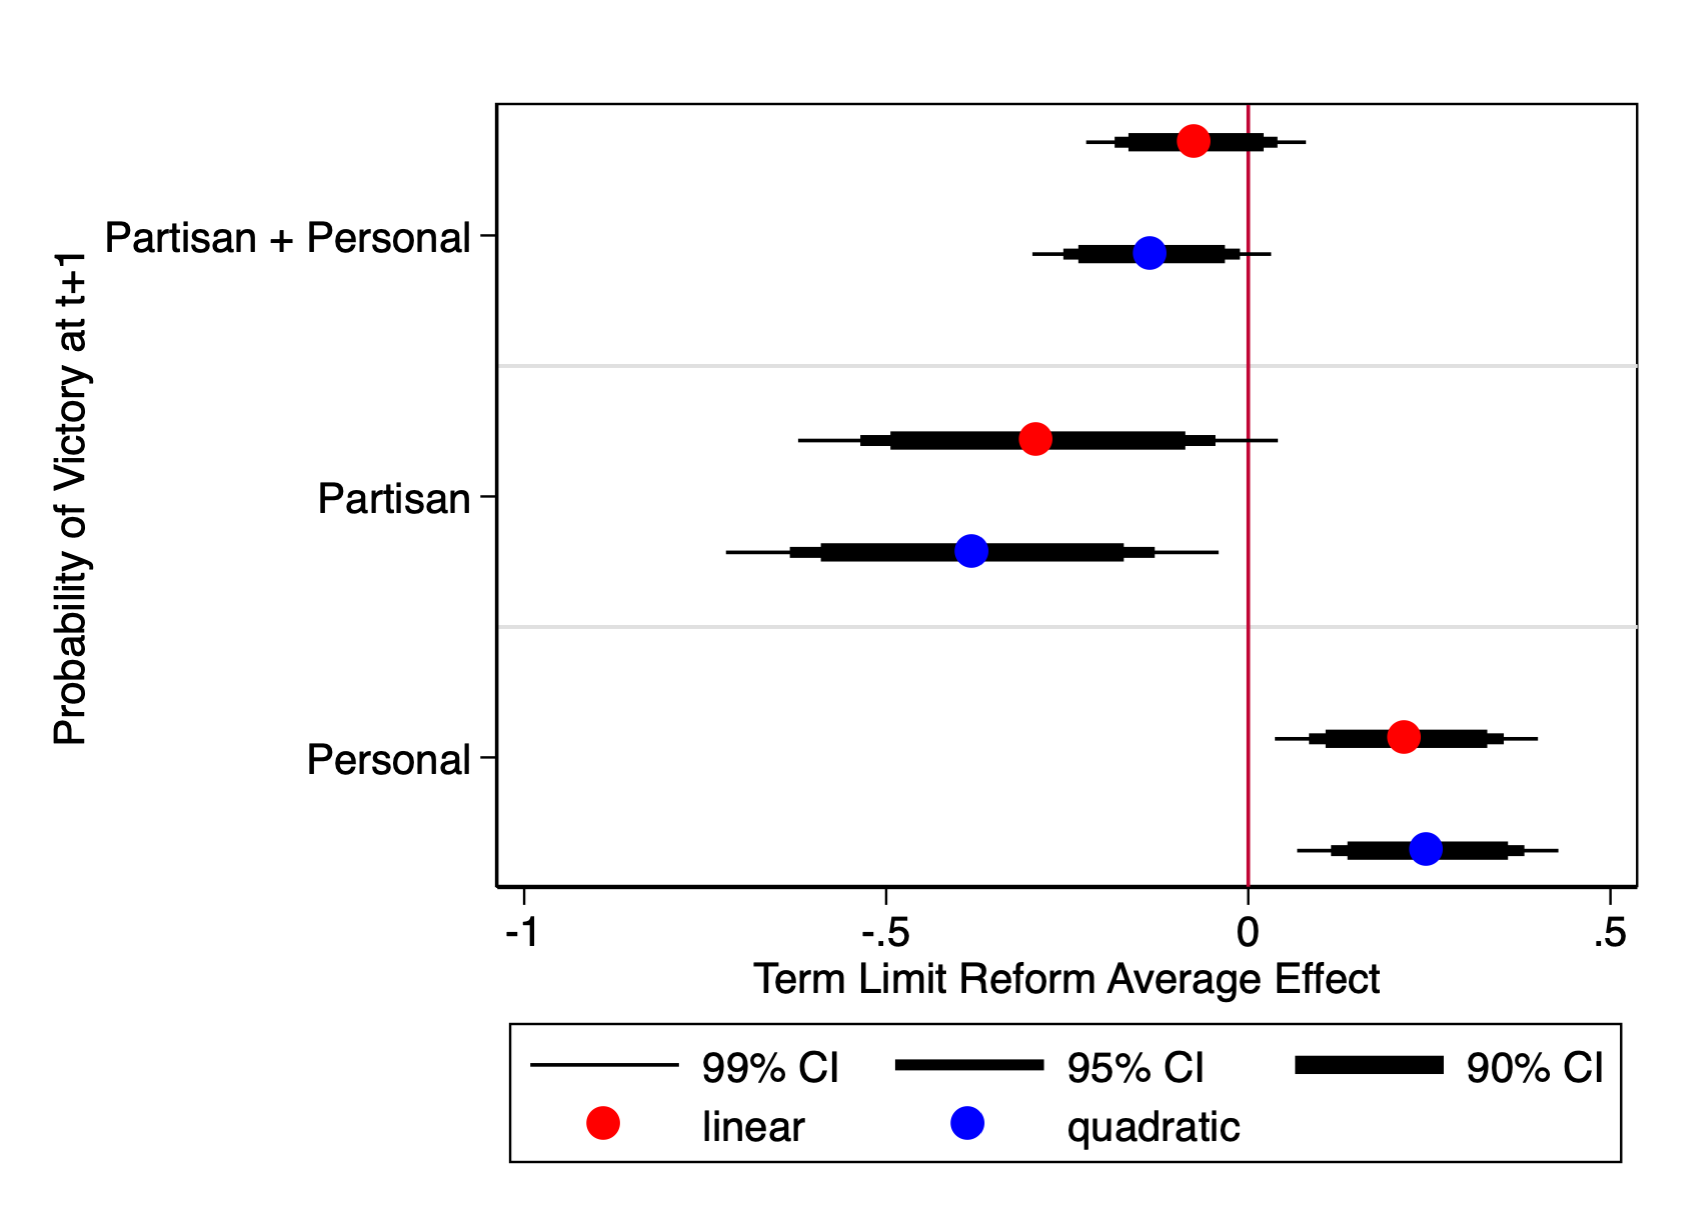
\includegraphics[width=0.9\textwidth]{../Figures_incumbency/partisan_personal_inc_advantage.png}
       \captionsetup{justification=centering}
       
 \textbf{Note:} Figure \ref{fig:main} shows the average treatment effect of the Term Limit Reform on the probability of winning in the following election using a difference in discontinuity of close elections design. This average effect was estimated using the IW estimators following \citet{abraham_sun_2020} for each lead and lag relative to the first year a municipality implemented reelection. Optimal bandwidths following \citet{calonicoetal_2014} are used. Red and blue points show that parallel trends hold, while hollow ones imply pretrends. 
\end{figure}  
   

\subsection{Identification assumptions} 

To validate causal effects three identification assumptions need to hold. First, cohort weighted specifications need to show parallel trends for both incumbency advantage measures. As seen in Figure \ref{fig:parallel_trend_main}  this is the case. Cohort weights further assure that parallel trends are not spurious due to correlation between the $k$ period indicators relative to treatment implementation.\footnote{Appendix Figure \ref{fig:naive_partisan&personal} find the same asymmetric effect as that of Figure \ref{fig:main} but no parallel trends are found when using a simple event study design.} Second, no anticipatory behavior from municipalities should be found; since we are only taking into account one election cycle post-treatment, we don't anticipate incumbents reacting in such a short time window. %[MISSING]%this is the case when running an ``event-to-event" analysis following \citet{cengiz_etal_2019}: there is no clustering in estimated coefficients on early and late state adopters.\footnote{Results available upon request.} 
Third, the design would be invalid if parties could manipulate close elections and sort themselves to those that imply a higher probability of winning. Two tests are commonly used to show validity on the design: (a) no covariate jump at the discontinuity on relevant pre-treatment variables and (b) density tests to see whether the number of municipalities above (or below) the cutoff threshold is significantly different from the number of municipalities below (or above). Appendix Figure \ref{fig:jump_covariates} shows evidence of no significant jump at the discontinuity of various pretreatment covariates including a dummy on the alignment with the President, alignment with the governor, logged population, a dummy of the party who was ruling the municipality one election before (PRI, PAN or MORENA/PRD), and the effective number of parties. Furthermore, Appendix Figure \ref{fig:mccrary} shows no density difference between municipalities just above and below the cutoff for the linear and polynomial specifications. 

 \begin{figure}[h]   
\centering
 \caption{Effect of Term Limit Reform on Incumbency Advantage \\ -difference-in-discontinuity of close elections-}
 \label{fig:parallel_trend_main}
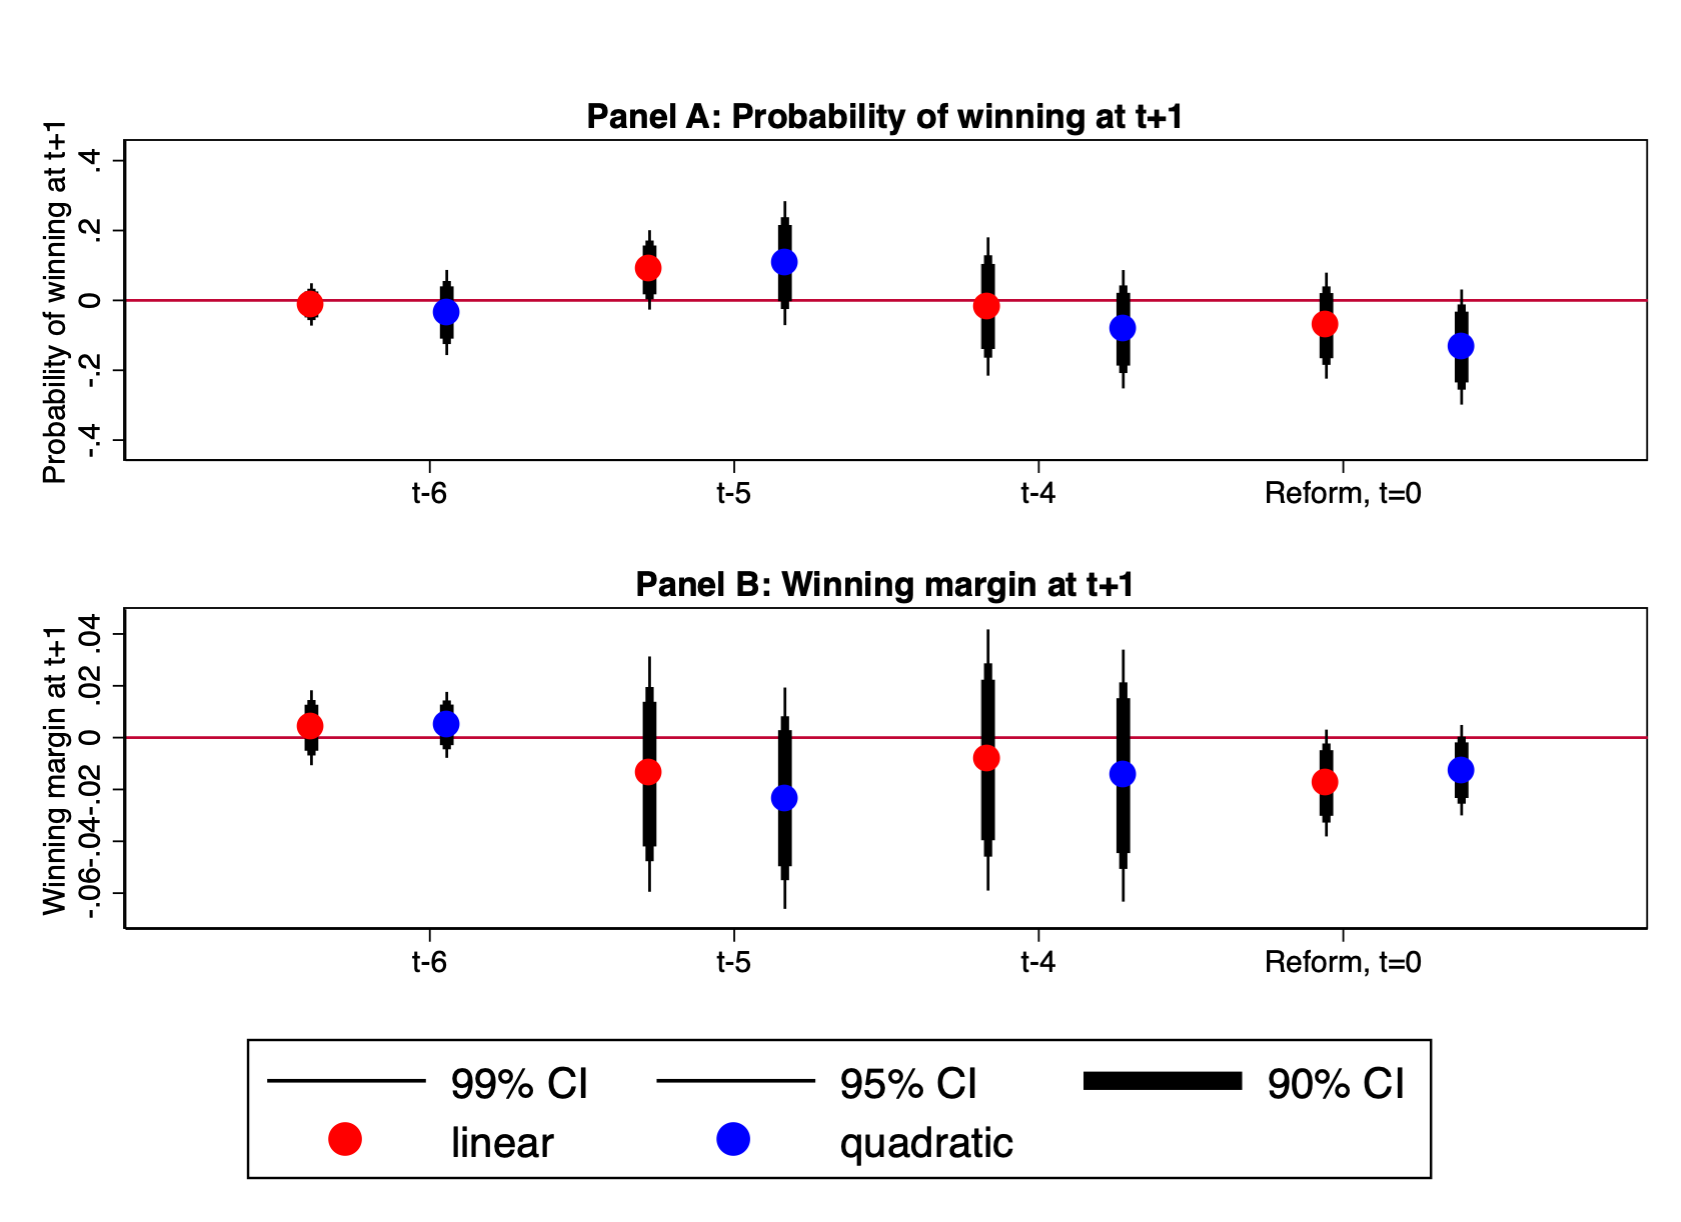
\includegraphics[width=0.9\textwidth]{../Figures_incumbency/parallel_trend.png}
       \captionsetup{justification=centering}
         
 \textbf{Note:} Figure \ref{fig:parallel_trend_main} shows the average treatment effect of the Term Limit Reform on the probability of winning in the following election using a difference in discontinuity of close elections design. This average effect was estimated using the IW estimators following \citet{abraham_sun_2020} for each lead and lag relative to the first year a municipality implemented reelection. Optimal bandwidths following \citet{calonicoetal_2014} are used.  
 
\end{figure}   
    
\subsection{Robustness tests \label{sec:robustness}}
  
To test the robustness of results I start by comparing the difference-in-discontinuity of close election design results from Section \ref{sec:results} with the design used by \citet{fowler_hall_2014}. To estimate the personal and partisan incumbency advantages they run two different regressions: first, a regression discontinuity design of close elections where candidates are prevented from running for reelection, i.e. they are term limited; second, a regression discontinuity design where candidates are non-term limited, i.e. they can run for reelection if desired. The difference between the estimated coefficients of these two models results in the personal incumbency advantage, while the first one estimates the partisan one and the second one the conjoint partisan and personal incumbency advantages. Results are then corrected by the probabilities of reelection attempts as described in Section \ref{sec:personal_vs_partisan}. Table \ref{tab:fowler_hall} shows the partisan and personal incumbency advantages following \citet{fowler_hall_2014} using both the probability of victory as well as the winning margin in the next election as outcomes. Panel A shows the results using a linear polynomial while Panel B uses a quadratic one. Overall, we see that without term limits, in Mexico incumbents had a positive but non-significant incumbency advantage. However, term limited races show that a partisan incumbency disadvantage exists between -8 to -9\% depending on the specification. Contrastingly, the difference between the term limit and non-term limit cases in column (3) shows the personal incumbency returns to be positive and significant to the 1\% level. These results coincide with the asymmetry found in Figure \ref{fig:main}. While estimates are half of those observed in that Figure, we need to consider that differences may arise from adjusting for heterogeneous treatment effects across the different treatment cohorts. 

For robustness we also check whether results change by varying the bandwidth for close elections. Appendix Figure \ref{fig:bandwidths} shows this to be the case overall, with an asymmetry found between the partisan and personal incumbency advantages for the linear and quadratic specifications. Moreover, across different bandwidths we observe the average incumbency returns to be non-different from zero speaking to the effect of reelection on incumbency returns due to a personal incumbency advantage. 
      
\begin{table}[htbp]\def\sym#1{\ifmmode^{#1}\else\(^{#1}\)\fi}
\centering
\caption{Personal and Partisan Incumbency Advantage following \citet{fowler_hall_2014}}
\label{tab:fowler_hall}
\scalebox{1}{
\begin{tabular}{lccc}
\hline \hline
& \multicolumn{3}{c}{\textbf{Panel A: linear polynomial}}\\
& \multicolumn{1}{c}{No term limits:} & \multicolumn{1}{c}{term limits:} & \multicolumn{1}{c}{difference:}\\
Advantage: & \multicolumn{1}{c}{personal + partisan} & \multicolumn{1}{c}{partisan} & \multicolumn{1}{c}{personal} \\
& \multicolumn{1}{c}{(1)} & \multicolumn{1}{c}{(2)} & \multicolumn{1}{c}{(3)} \\
\cmidrule(lrr){2-2}  \cmidrule(lrr){3-3} \cmidrule(lrr){4-4}\\
\addlinespace
RD estimate: prob(victory in t+1) &      $ 0.0568^{} $ &  $ -0.1269^{***} $  &  $ 0.1468^{***} $  \\
& ($ 0.0508$) & ($ 0.0208 $)  & ($ 0.0038 $)\\
RD estimate: vote share in t+1 &      $ 0.0245^{} $ &  $ -0.0529^{***} $  &  $ 0.0618^{***} $  \\
& ($ 0.0243$) & ($ 0.0073 $)  & ($ 0.0024 $)\\
\addlinespace
Observations: prob(victory in t+1)      &            1257        &     9180  \\
Observations: vote share in t+1      &            1221        &     8758  \\
\\
& \multicolumn{3}{c}{\textbf{Panel B: quadratic polynomial}}\\
& \multicolumn{1}{c}{No term limits:} & \multicolumn{1}{c}{term limits:} & \multicolumn{1}{c}{difference:}\\
Advantage: & \multicolumn{1}{c}{personal + partisan} & \multicolumn{1}{c}{partisan} & \multicolumn{1}{c}{personal} \\
& \multicolumn{1}{c}{(1)} & \multicolumn{1}{c}{(2)} & \multicolumn{1}{c}{(3)} \\
\cmidrule(lrr){2-2}  \cmidrule(lrr){3-3} \cmidrule(lrr){4-4}\\
\addlinespace
RD estimate: prob(victory in t+1) &      $ 0.0442^{} $ &  $ -0.1291^{***} $  &  $ 0.1384^{***} $  \\
& ($ 0.0676$) & ($ 0.0258 $)  & ($ 0.0042 $)\\
RD estimate: vote share in t+1 &      $ 0.0311^{} $ &  $ -0.0510^{***} $  &  $ 0.0656^{***} $  \\
& ($ 0.0274$) & ($ 0.0092 $)  & ($ 0.0026 $)\\
\addlinespace
Observations: prob(victory in t+1)      &            1257        &     9180  \\
Observations: vote share in t+1      &            1221        &     8758  \\
\hline \hline
\multicolumn{4}{p{1\textwidth}}{\footnotesize{Notes: Standard errors in parentheses are clustered at the state level, with the following significance-level: $^{***}$ 1\%; $^{**}$ 5\%; and $^*$ 10\%, that refer to two-sided t-test with the null hypothesis equal to 0 for each relative time period. Table estimated using all elections since the year 2000.}}
\end{tabular}
}
\end{table}
   


\section{Mechanisms: What explains the observed electoral returns from incumbency? \label{sec:mechanisms}}
           
A big concern of the literature has been understanding the determinants of incumbency advantage. To date, we can identify at least three broad types of explanations. First, what incumbents do (and opponents cannot do) emphasizing the resources, visibility, and power that incumbents gain from office holding \citep{mayhew_1974, fiorina_1989, king_1991, cox_morgensten_1993}.  Second, quality-based explanations that emphasize who incumbents are (and who their opponents are) \citep{cox_katz_1996, levitt_wolfram_1997, ansolabehere_snyder_2000, eggers_2017}. In this second line we find explanations related to incumbents’ quality as well as the “scare-off effect”, or the ability incumbents have to scare off high-quality challengers. A third and more recent type of mechanism emphasizes the role of information. \citet{ashworth_bdm_2008} find that incumbency advantage is dependent on how precise the information is about incumbent’s ability to voters. More recently, \citet{ashworth_etal_2019} expand on the role of information to explain incumbency advantage: through a theoretical model, they show that incumbents have an additional information advantage to challengers: they govern while challengers do not. This is so even absent any partisanship, electoral selection or challenger scare off. However, to date there is no empirical identification of the information-based explanation proposed by these authors. Moreover, if theoretical work done by Ashworth and co-authors is correct, all other explanations of incumbency advantage might be biased by the role information plays. 

To test if a resource-based incumbency advantage explains the returns observed in Section \ref{sec:results}, I evaluate the effect of the reform on municipal revenues and fiscal transfers. Local tax revenues have been widely use to proxy for incumbents effort on state capacity building. The most relevant tax revenues at the municipal level in Mexico are property and estate taxes. Two additional sources of local revenues are important, those coming from the ownership of vehicles (\emph{tenencia} in Spanish) as well as revenues from taxing new cars. Mayors tend to use these two sources of revenues to increase their treasury but are highly unapproved by voters. As a result, we would expect mayors with reelection incentives not to rely on these types of tax revenues. Figure \ref{fig:revenues1} Panel A shows that total municipal revenues increased during the first years of office from $t$ to $t+3$. A large increase of municipal revenues comes from an increase in tax revenues (Figure \ref{fig:revenues1} Panel B), particularly property and estate tax revenues (Panel C and D), and a lower proportion from the increase in tax revenues from production, consumption and transactions (but these estimates are non-significant; see Figure \ref{fig:revenues2} Panel E). Interestingly, unpopular taxes like the \emph{tenencia} and those on new cars show a decrease in revenues the first year in office, and for the tenencia the three years afterwards. All these estimates show parallel trends and consider only the subsample of municipalities used to estimate Figure \ref{fig:main}. 
  
  
\begin{figure}[h]   
\centering
 \caption{Effect of Term Limit Reform on Municipal Revenues}
 \label{fig:revenues1}
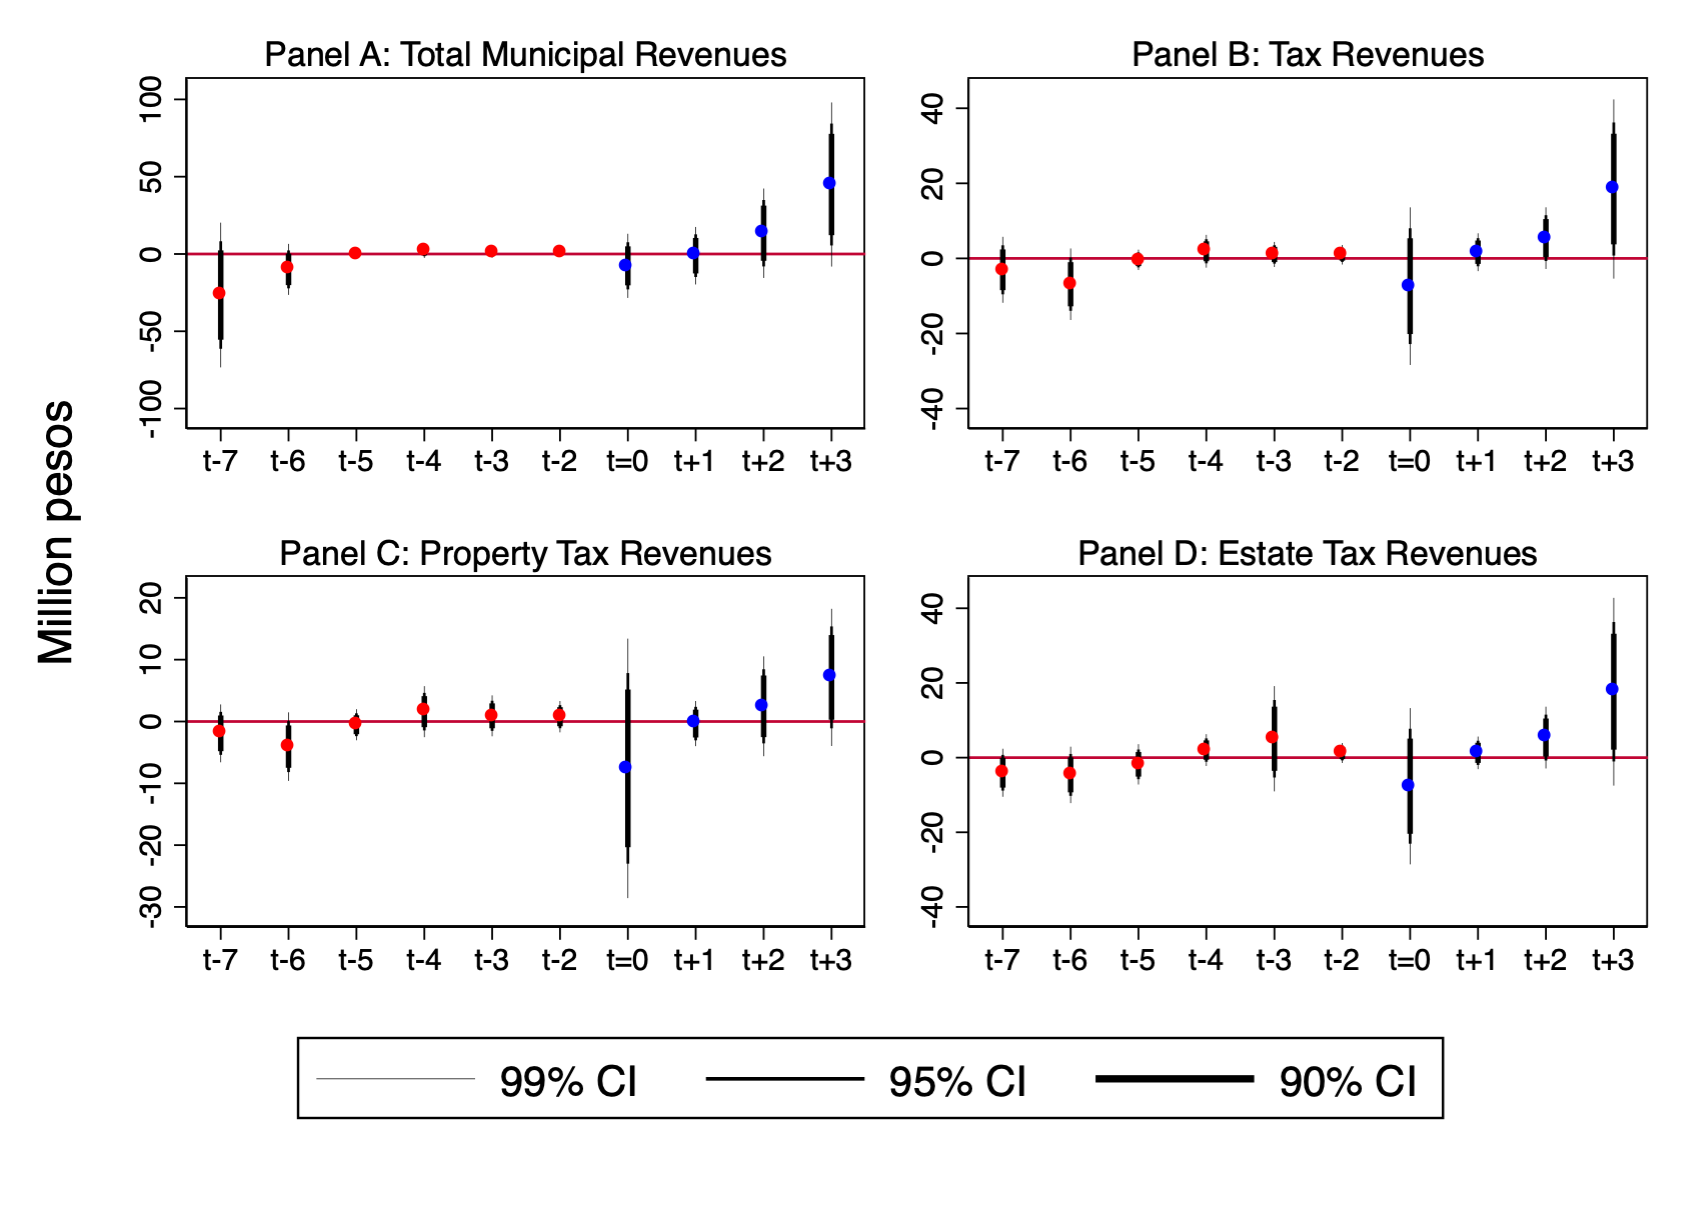
\includegraphics[width=0.9\textwidth]{../Figures_incumbency/revenues_allyears1.png}
       \captionsetup{justification=centering}
         
 \textbf{Note:}  Figure \ref{fig:revenues1} shows the average treatment effect of the Term Limit Reform on different measures of municipal revenues. This average effect was estimated using the IW estimators following \citet{abraham_sun_2020} for each lead and lag relative to the first year a municipality implemented reelection. Same optimal bandwidths as those in Figure \ref{fig:main} are used, as well as the same municipalities. All variables are deflated and in million pesos. 
\end{figure}   

\begin{figure}[h]   
\centering
 \caption{Effect of Term Limit Reform on Municipal Revenues (continuation)}
 \label{fig:revenues2}
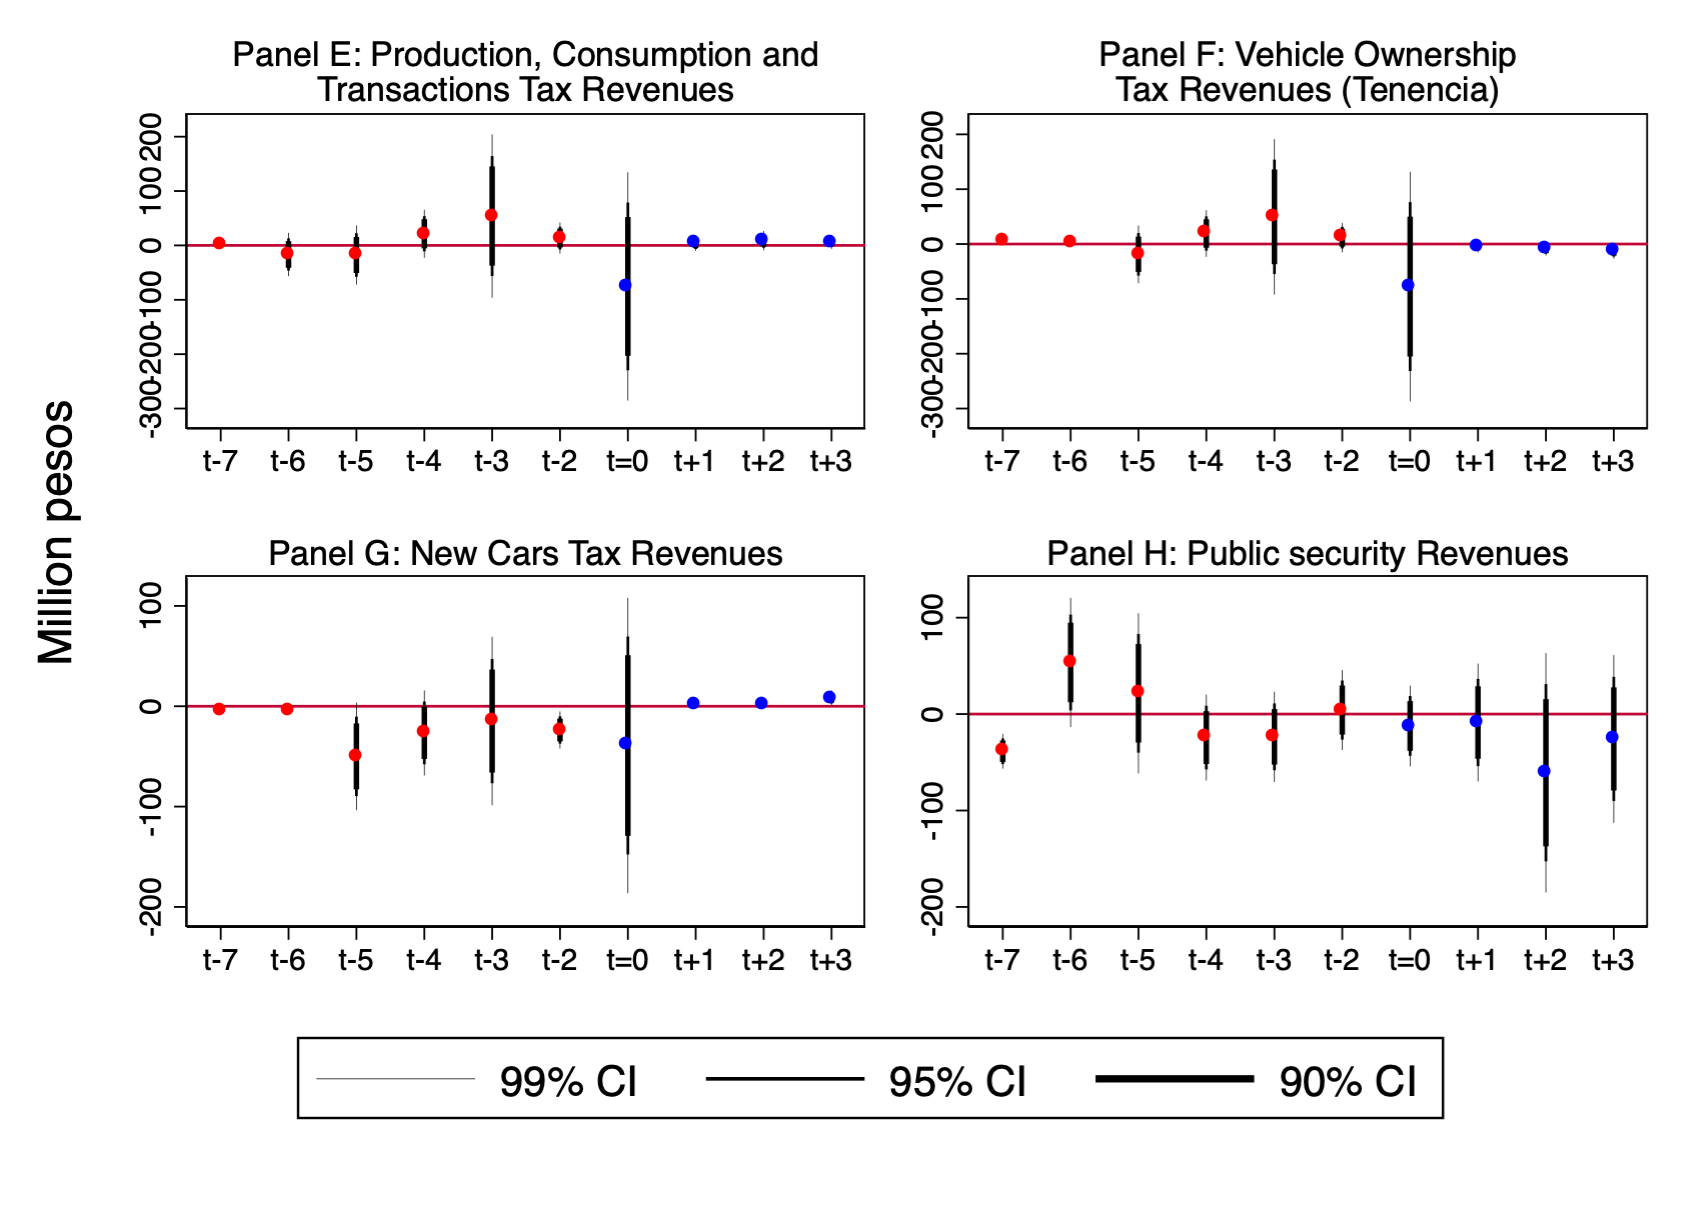
\includegraphics[width=0.9\textwidth]{../Figures_incumbency/revenues_allyears2.png}
       \captionsetup{justification=centering}
         
 \textbf{Note:} Figure \ref{fig:revenues2} shows the average treatment effect of the Term Limit Reform on different measures of municipal revenues. This average effect was estimated using the IW estimators following \citet{abraham_sun_2020} for each lead and lag relative to the first year a municipality implemented reelection. Same optimal bandwidths as those in Figure \ref{fig:main} are used, as well as the same municipalities. All variables are deflated and in million pesos.  
          
\end{figure}  

 Besides revenues, we can use data on municipal transfers from the federation or the state to proxy for resources. These transfers can be divided into two types: labeled and unlabeled. Labeled transfers are those which are determined mostly by the use of fiscal formulas and are targeted to specific ``labeled'' expenses or conditional on certain activities. The most prominent municipal transfer in Mexico si the Federal and State Contributions Fund. Unlabeled transfers are those that municipalities can exercise freely and are generally not audited by Federal Superior Audit in Mexico. The most prominent ones include the General Participation Fund as well as secondary participating funds. Other relevant unlabelled municipal transfers are the Municipal Development Fund, the Contribution Fund to Strengthen Municipalities and the Contribution Fund for Municipal Social Infrastructure. Figure \ref{fig:resources2} shows the effect of the Term Limit Reform on these transfers. We see an increase of participations (Panels A and B), as well as municipal funds (Panels C and D) in municipalities where mayors can run for reelection relative to those that are term limited. Interestingly, the increase is particularly salient four years after the implementation of the reform, i.e. in the first year of reelection. In contrast, no effects are found for labeled transfers (Panel F). 
   
 \begin{figure}[h]   
\centering
 \caption{Effect of Term Limit Reform on Transfers from the Federation or the State}
 \label{fig:resources2}
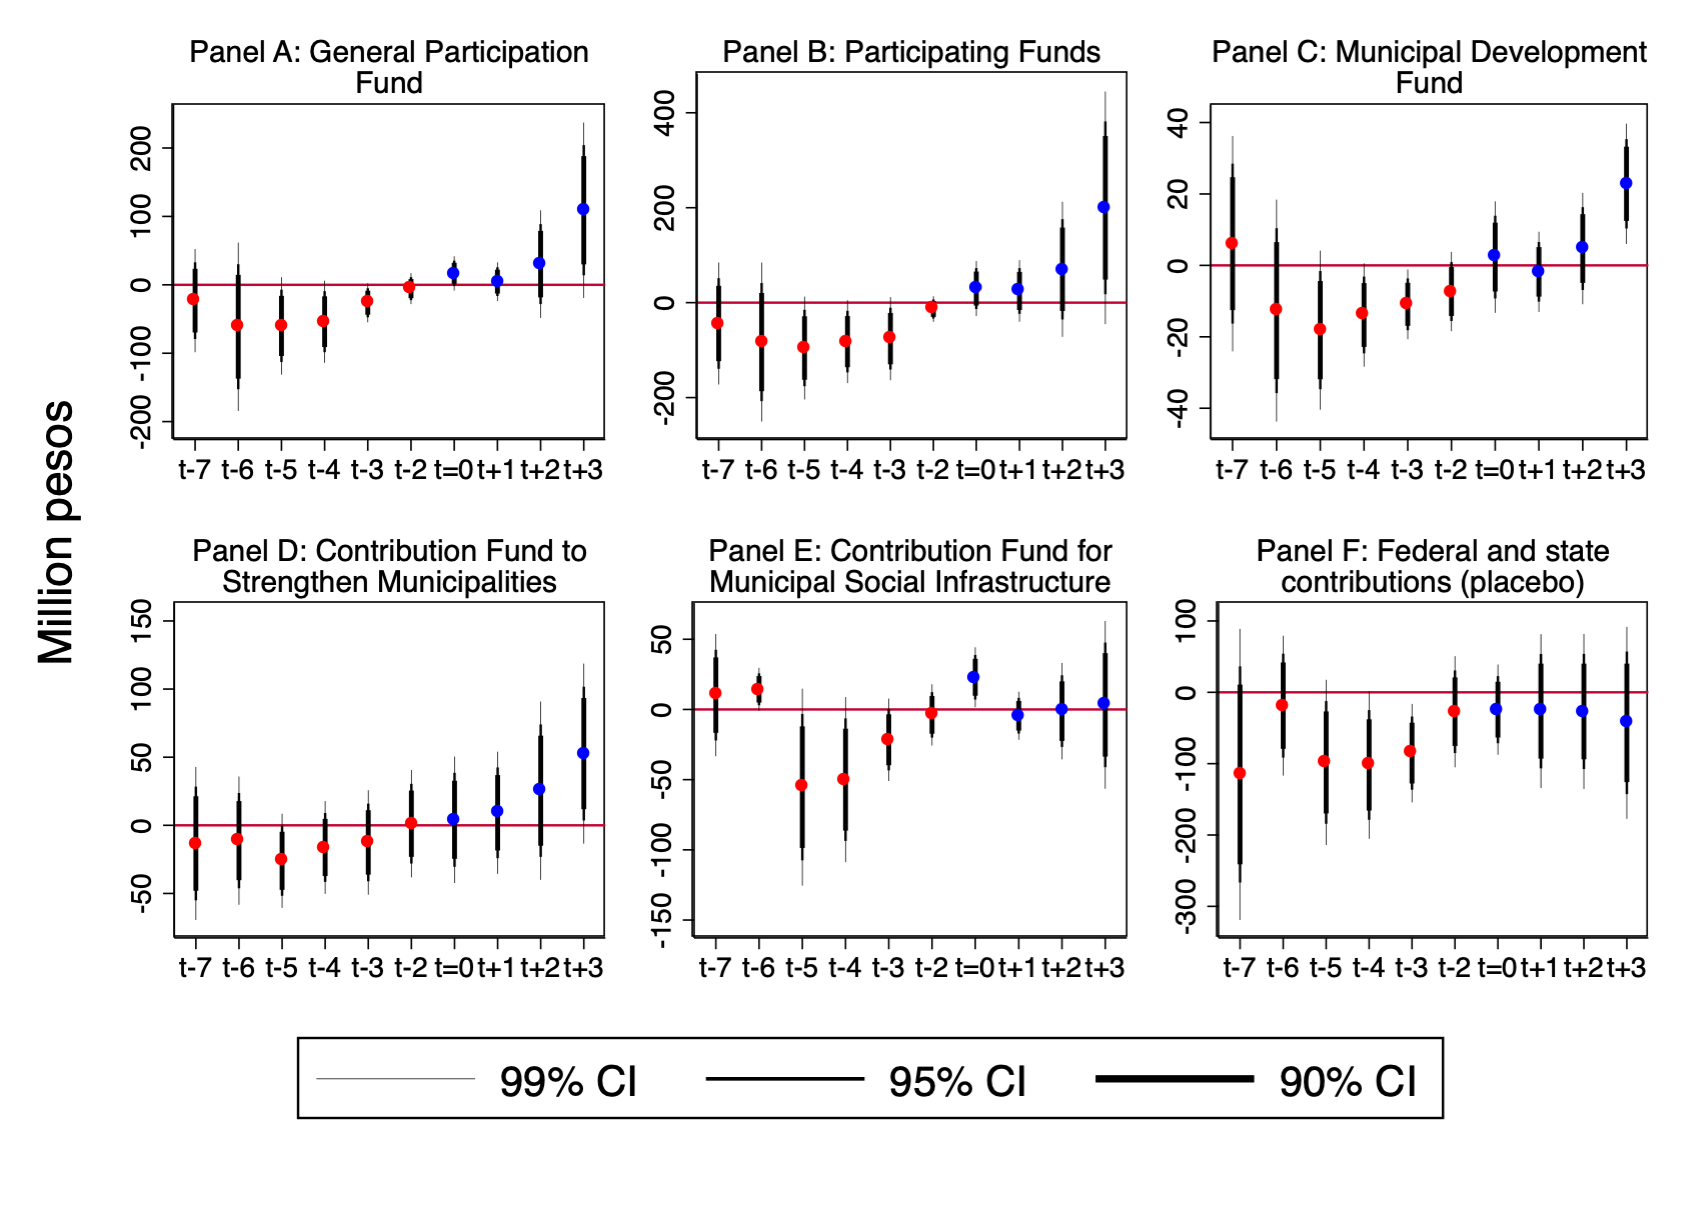
\includegraphics[width=0.9\textwidth]{../Figures_incumbency/resouce_based_incumbency_allyears.png}
       \captionsetup{justification=centering}
         
 \textbf{Note:} Figure \ref{fig:resources2} shows the average treatment effect of the Term Limit Reform on various transfers measures. This average effect was estimated using the IW estimators following \citet{abraham_sun_2020} for each lead and lag relative to the first year a municipality implemented reelection. Same optimal bandwidths as those in Figure \ref{fig:main} are used, as well as the same municipalities. All variables are deflated and in million pesos.   
       
\end{figure}  

Both transfers and revenues are used to proxy for measures of the resources incumbents may get and may affect their reelection chances or that of their parties. This is called the resource-based incumbency advantage where citizens create a positive incumbency return expecting a higher budget or transfer in the future \citep{cox_morgensten_1993}. The literature has also used measures of casework services to constituents or the ability to expand the bureaucracy and thus public labor to test for a resource based incumbency advantage \citep{cox_katz_1996}. I rely on data from the Municipal Government Census (\emph{Censos de Gobierno Municipal}) from 2011 to 2019 which collect information on the number of bureaucrats of municipalities, as well as the number of city council sessions, the number of approved initiatives of law and the percentage of municipal budget spend, all in the year prior to the census. This data spans from 2010 to 2018 every two years. For the case of Mexico, council sessions and initiatives approved is performed by the local council members (\emph{regidores}) who are elected by proportional representation in mayoral elections according to the vote received by the mayor. As such, they work directly with the mayor and can be considered as his bureaucrats specially when they belong to the same party. Figure \ref{fig:effort} shows the effect of the 2014 Term Limit Reform on these measures. As with Figure \ref{fig:main}, the election prior to reform, i.e. $t-3$ serves as the baseline period of comparison. Overall we find no difference in the number of city council sessions (Panel A), approved initiatives of law (Panel B), nor the number of bureaucrats (Panel D) between municipalities with term-limited and non-term limited mayors. Furthermore, the percentage of budget spend serves as a proxy of effort as municipal mayors in Mexico tend not to spend their resources during their tenure, the so called \emph{subejercicios} in Spanish. It seems mayors up for reelection hold \emph{subejercicios} of 10\% of the total budget, but a seemingly decreasing trend calls for further robustness. In conclusion, taking into account the evidence provided by municipal revenues, transfers and other measures of resources available to mayors up for reelection, we find evidence of a resource-based incumbency advantage.


 \begin{figure}[h]   
\centering
 \caption{Effect of Term Limit Reform on Other Resources}
 \label{fig:effort}
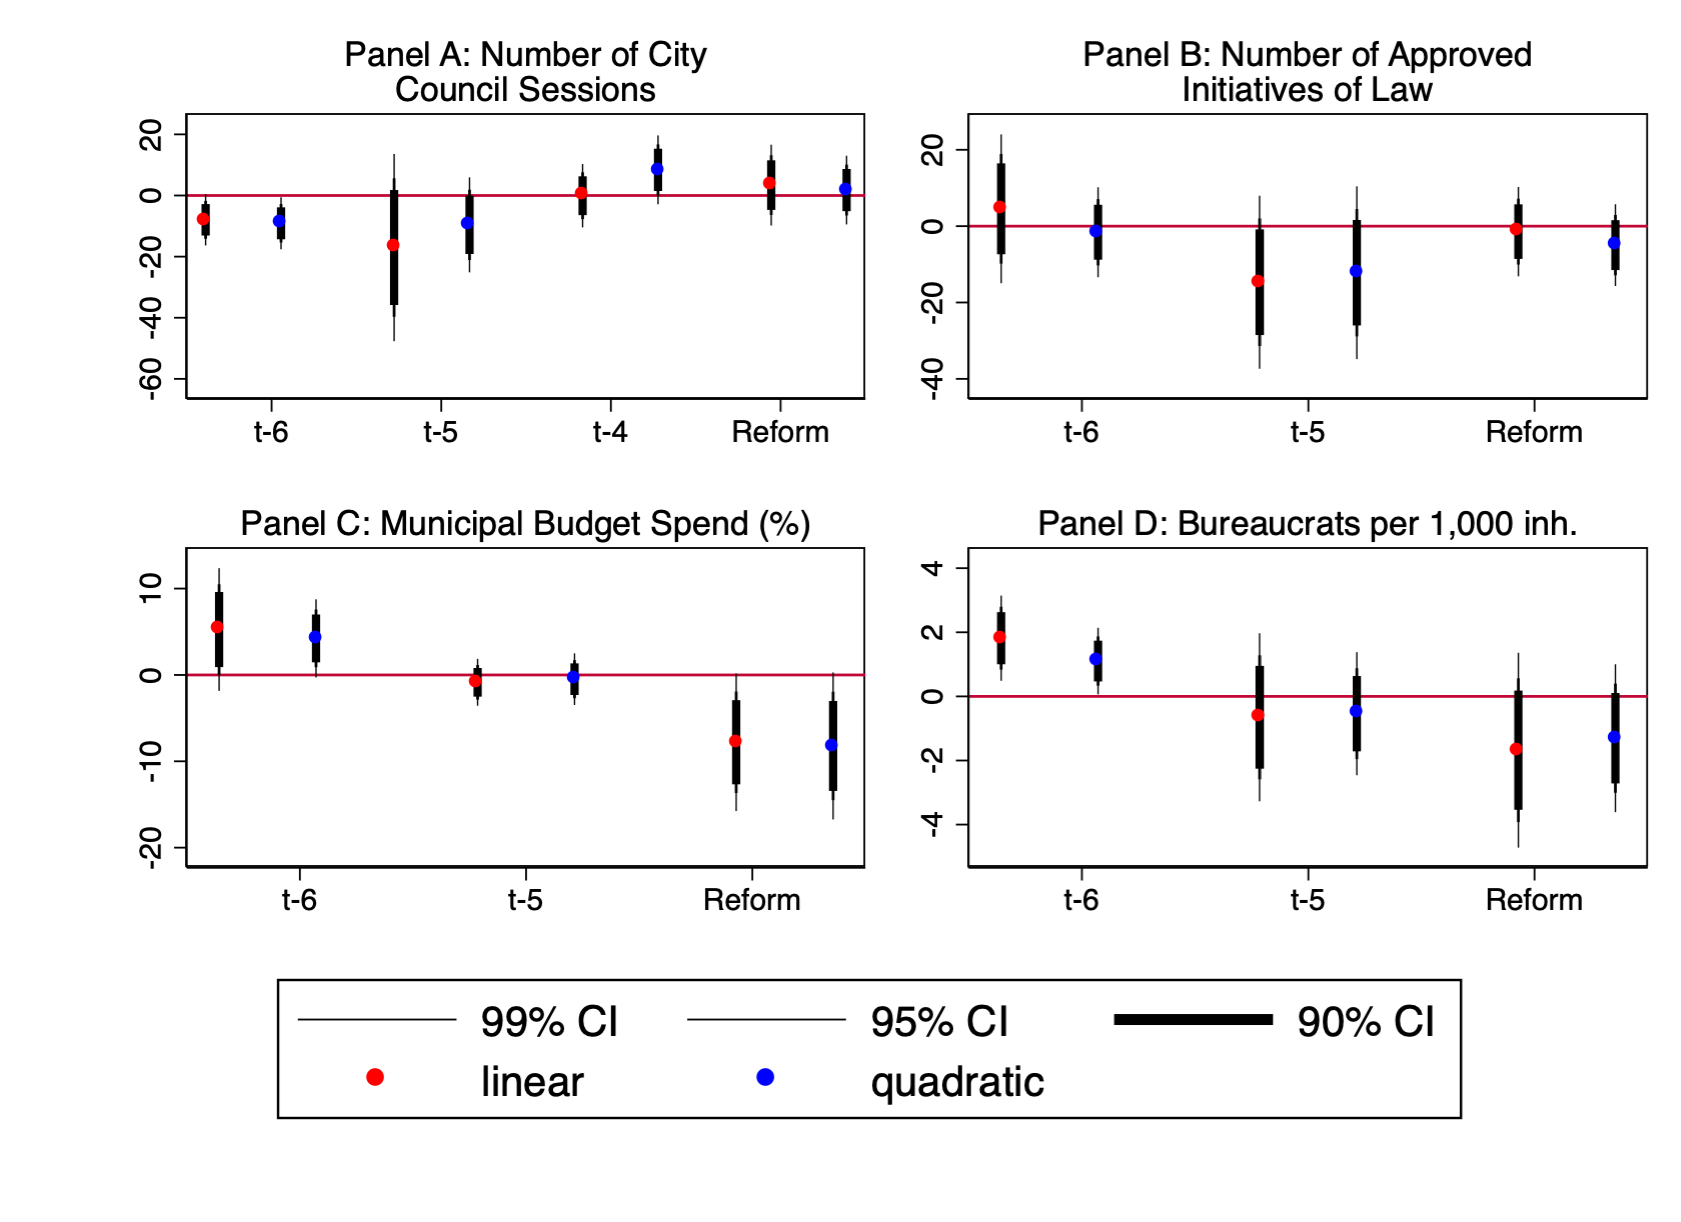
\includegraphics[width=0.9\textwidth]{../Figures_incumbency/effort_based_incumbency.png}
       \captionsetup{justification=centering}
         
 \textbf{Note:} Figure \ref{fig:effort} shows the average treatment effect of the Term Limit Reform on various transfers measures. This average effect was estimated using the IW estimators following \citet{abraham_sun_2020} for each lead and lag relative to the first year a municipality implemented reelection. Same optimal bandwidths as those in Figure \ref{fig:main} are used, as well as the same municipalities.   
\end{figure}   

 \begin{figure}[h]   
\centering
 \caption{Effect of Term Limit Reform on the Quality of Candidates}
 \label{fig:quality_trend}
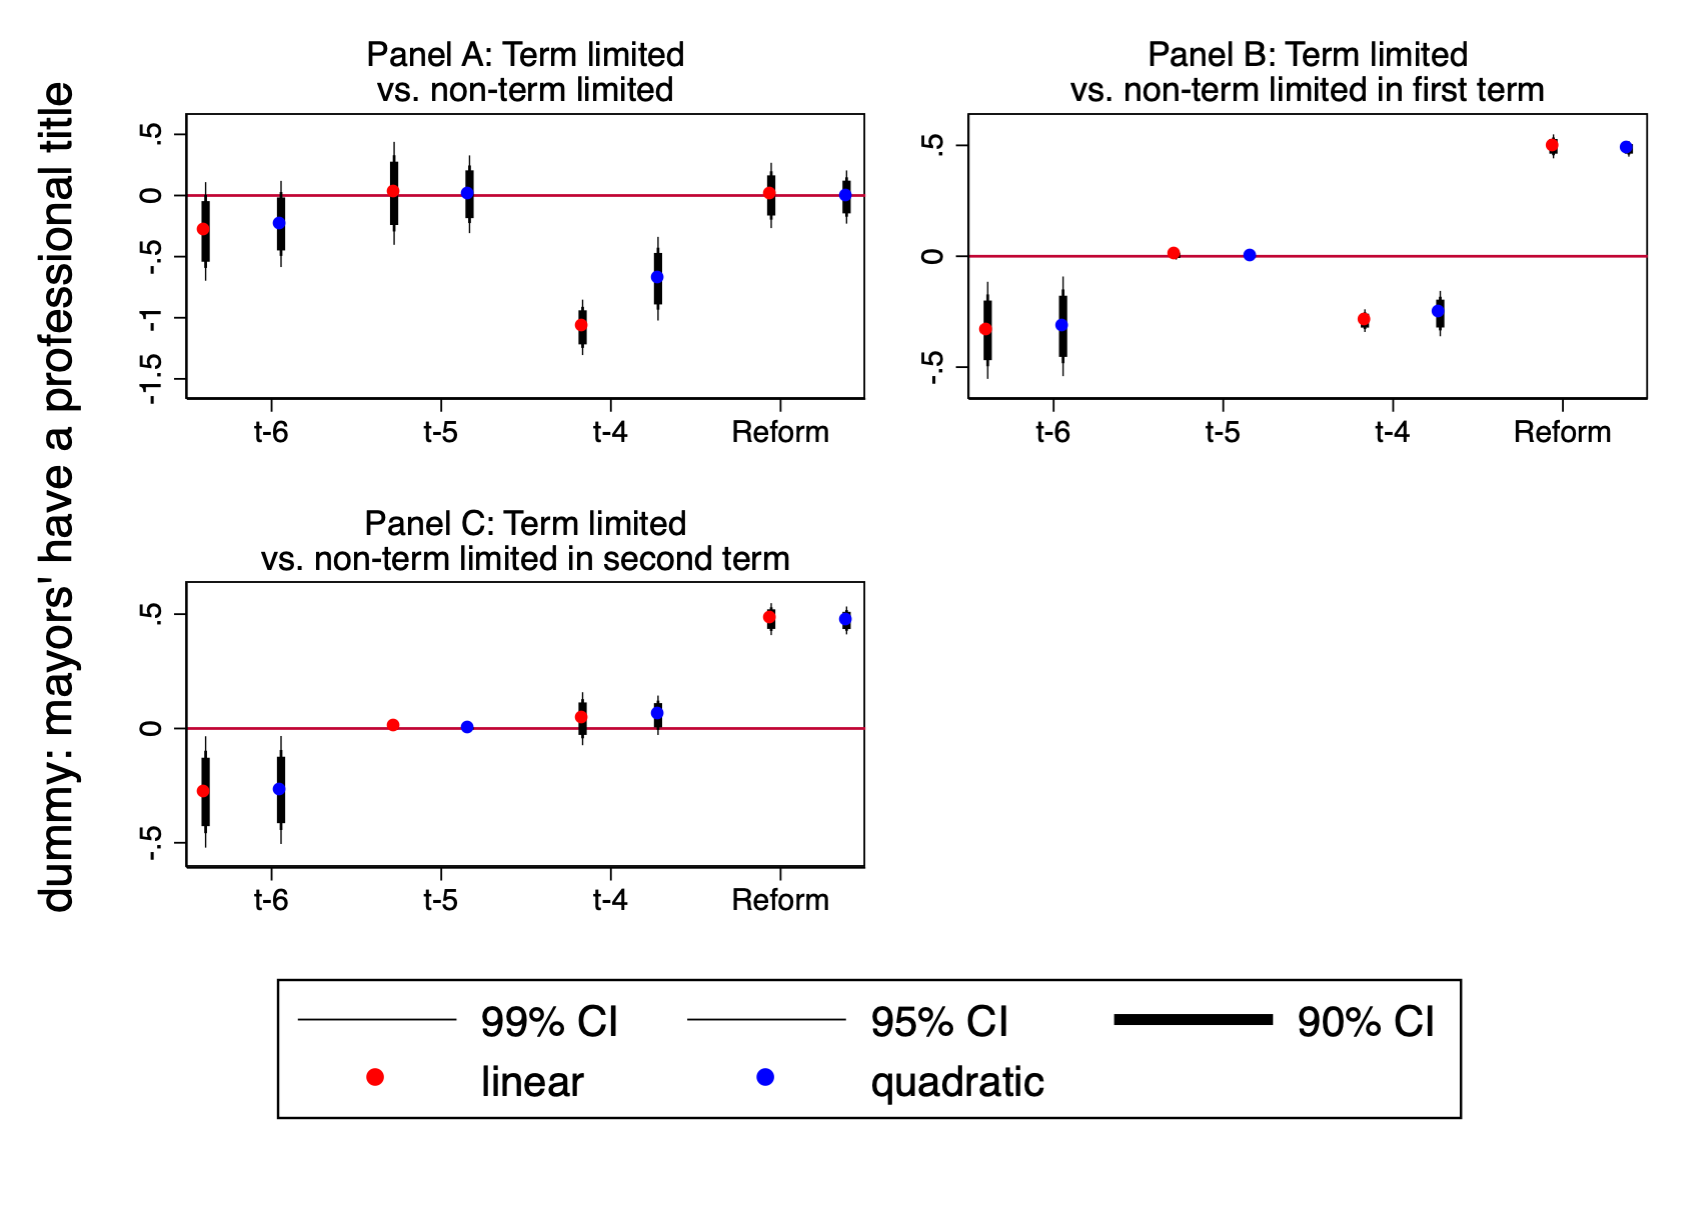
\includegraphics[width=0.9\textwidth]{../Figures_incumbency/quality_parallel.png}
       \captionsetup{justification=centering}
         
 \textbf{Note:} Figure \ref{fig:quality_trend} shows the average treatment effect of the Term Limit Reform on a dummy indicator of whether candidates hold a professional title. This average effect was estimated using the IW estimators following \citet{abraham_sun_2020} for each lead and lag relative to the first year a municipality implemented reelection. Same optimal bandwidths as those in Figure \ref{fig:main} are used, as well as the same number of observations.   
     
\end{figure}   
To test for a quality-based incumbency advantage, Figure \ref{fig:quality_trend} shows the difference-in-discontinuity of close elections specification on the effect of the term limit reform on the quality of candidates measured as a dummy indicator of whether incumbents hold a professional degree. Panel A compares term limited vs. non-term limited incumbents as done in Figure \ref{fig:main}. We observe no difference in the quality of incumbents, but pretrends are found in $t-4$. Panel B and C carry on a different experiment. Panel B compares term limited to non-term limited incumbents in their first term only. While incumbents up for reelection tend to hold more professional degrees than term limited ones, pretrends reduce the assurance of this claim. Lastly, besides differences in the quality of incumbents there could exist a difference in the quality of challengers who out of fear to the experience and ability of incumbents might choose not to run for office, the so called scare-off effect. Sadly, there is no municipal level data on the quality of challengers. However, in Panel C we develop an experiment that could proxy such decision: we compare term limited to non-term limited incumbents in their second term. The idea is that if a scare-off effect exists we should observe term limit incumbents differ in their quality relative to those with more experience and ability, i.e. those incumbents who reelected and are in their second term. Panel C shows this difference to be substantial, close to 50\% and significant to the 1\% level. Parallel trends hold for $t-4$ and $t-5$, but a difference exists when comparing elections six years prior ($t-6$), i.e. two elections before for the majority of races in $t$. Overall, given the existence of pretrends, we cannot rule out the possibility of a quality-based incumbency advantage. Results, however, suggest a potential scare-off effect might be taking place. 

Lastly, these estimates do not allow to test for an information-based incumbency advantage. To do so we would need data on whether citizens increased their information reception of incumbents actions and behavior in office. Future work is needed to disentangle the specific information and quality-based mechanisms behind the observed incumbency returns in mayoral elections in Mexico. 

  

\section{Conclusion} 

This paper disentangles the partisan from the personal incumbency advantages. By not disentangling these two concepts when estimating incumbency electoral returns, most of the literature has failed to correctly identify the valuation citizens have on the electoral system and the existent accountability dynamics. To unbox incumbency advantage into its personal and partisan components, this paper relies on a difference-in-discontinuity of close elections design that exploits the staggered implementation of the 2014 Electoral Reform in Mexico that removed term limits for local mayors. Term limit mayors allows us to identify the partisan incumbency returns, while those up for reelection identify both the partisan and personal returns. The difference between these two measures allows for the identification of the personal incumbency advantage. Moreover, the difference-in-difference setup allows us to test for no differential trends of these two type of races prior to the introduction of the reform, while the regression discontinuity of close elections design allows us to reduce the potential of omitted variables, including party, elections and candidates differences. Lastly, we consider only mayors in their first terms which allows us to leave aside concerns coming from differences in experience and skills. 

The main result of the paper shows that the implementation of reelection in Mexico led to an incumbency disadvantage. However, this incumbency disadvantage can be decomposed into a personal incumbency \emph{advantage} and a partisan incumbency  \emph{disadvantage}. Moreover, the observed incumbency disadvantage with reelection is lower than the partisan incumbency disadvantage before reelection, making the personal incumbency advantage the primary reasons behind the decrease in the disadvantage for mayoral incumbents. These results imply that reelection makes incumbency a personal affair and not only a partisan one, and may signal a potential party dealignment in Mexican politics. The asymmetric effects also imply parties in Mexico do not hold a credible threat to punish renegade mayors, and may be punished harshly by citizens by not doing so. 

The paper further tries to explain the reasons behind the observed incumbency returns. An increase in the revenues and fiscal transfers to municipalities provide strong evidence of a resource-based incumbency advantage. In other words, citizens create a positive incumbency return with candidates who they expect will bring a higher budget or transfer in the future, and not their parties. We also test whether a quality-incumbency advantage exists, including a potential scare-off effect where high quality challengers may not choose to compete given the advantage incumbents may hold. While no quality differences are found between term limit and non-term limit incumbents, and a scare-off effect seems to exist, the existence of pretrends clouds this conclusion. It is important to acknowledge that to further prove this mechanism more data on the quality of incumbents and challengers in mayoral elections in Mexico is needed. It is also important to note that we do not have data on whether citizens increased their information reception of incumbents action, data that could be used to test whether an information-based incumbency advantage explains the observed results. 




\clearpage               
%APPENDIX -----------------------------------------------

%%%%%%%%%%%%
\bibliographystyle{aer} 
\bibliography{References}    

\clearpage
%APPENDIX -----------------------------------------------
\begin{appendix}

%%%%%%%%%%%%%%%%%%%%%%%%%%%%%%%%% 

\section{Tables and Figures \label{appendix:tables_figures}}
 
\renewcommand{\thetable}{A-\arabic{table}}
\setcounter{table}{0}
 
\renewcommand{\thefigure}{A-\arabic{figure}}
\setcounter{figure}{0}
%%%%%%%%%%%%%%%%%%%%%%%
%Table
\begin{table}[H]
\centering 
\caption{Descriptive statistics}
 
\label{tab:descriptive}
\scalebox{0.75}{ 
{
\def\sym#1{\ifmmode^{#1}\else\(^{#1}\)\fi}
\begin{tabular}{l*{1}{ccccc}}
\hline\hline
            &        \textbf{Mean}&  \textbf{SD}&  \textbf{Min}&  \textbf{Max}& \textbf{N}\\
\hline    
\emph{Pane A - Incumbency Advantage:} 	&		&		&		&		\\
Probability of winning, election at t+1&        0.40&        0.49&           0&           1&       2,247\\
Vote share, election at t+1&       -0.05&        0.18&          -1&         .59&       2,246\\

\\
\emph{Panel B - Controls and Forcing Variable:} 	&		&		&		&		\\
Winning margin: first - second runner (governor)&        0.17&        0.14&           0&           1&       2,227\\
alignment with federal executive=1; 0 otherwise&        0.75&        0.43&           0&           1&       2,227\\
alignment with state executive=1; 0 otherwise&        0.37&        0.48&           0&           1&       2,227\\
Winning margin: first - second runner&        0.08&        0.05&           0&           1&       2,227\\
PAN mayor=1; 0 otherwise&        0.33&        0.47&           0&           1&       2,227\\
PRI mayor=1; 0 otherwise&        0.49&        0.50&           0&           1&       2,227\\

Population (INEGI and CONAPO projections)&      49,233&     129,415&         409&   1,714,709&       2,247\\


\\
\emph{Panel C - Mechanisms-Fiscal Transfers:} 	&		&		&		&		\\
General Participations Fund (Mill. pesos)&          39&          94&         .81&       1,221&       1,638\\
Participating Fund (Mill. pesos)&          52&         127&         .21&       1,498&       1,656\\
Municipal Development Fund (Mill. pesos)&         9.7&          24&          .2&         345&       1,642\\
Federal and state contributions (Mill. pesos)&          60&         131&        .048&       2,133&       1,768\\
Contribution Fund for Municipal Social Infrastructure (Mill. pesos)&          18&          30&        .048&         618&       1,759\\
Contribution Fund to Strengthen Municipalities (Mill. pesos)&          23&          61&         .15&         865&       1,755\\

\\
\emph{Panel D - Mechanisms-Municipal Revenues:} 	&		&		&		&		\\
Total Municipal Revenues (Mill. pesos)&         166&         420&           2&       5,715&       1,779\\
Tax Revenues (Mill. pesos)&          19&          82&      .00017&       1,256&       1,735\\
Property Tax Rrevenues (Mill. pesos)&          12&          48&      .00013&         476&       1,360\\
Estate Tax Revenues (Mill. pesos)&          17&          66&      .00013&         672&       1,506\\
Prod., Cons. and Trans. Tax Revenues (Mill. pesos)&         1.2&          19&     .000096&         488&         671\\
Vehicle Ownership Tax Revenues (Mill. pesos)&          .5&         1.9&     .000081&          29&       1,324\\
New Cars Tax Revenues (Mill. pesos)&         .87&         2.9&       .0032&          49&       1,530\\
Public Security Revenues (Mill. pesos)&         6.1&          15&     .000078&         121&         211\\

\\
\emph{Panel E - Mechanisms-Other Resources:} 	&		&		&		&		\\
Number of City Council Sessions&          23&          19&           0&         288&       1,784\\
Number of Approved Initiatives of Law&          17&          32&           0&         295&         884\\
Percentage of Municipal Budget Spend&          11&          15&           0&         100&         789\\
Bureaucrats per 100,000 inhabitants&       1,945&       2,601&           0&      24,528&       1,247\\

\\
\emph{Panel F - Mechanisms-Incumbents' quality:} 	&		&		&		&		\\
Incumbent undergraduate or graduate title (indicator)&        0.11&        0.31&           0&           1&       2,148\\

\\ 

\hline\hline
\end{tabular} 
}
}
\end{table} 
   
\clearpage

%Table   
\begin{table}[htbp]\def\sym#1{\ifmmode^{#1}\else\(^{#1}\)\fi}
\centering
\caption{Difference-in-Discontinuity in close elections model: Effect of 2014 Term Limit Reform on Incumbency Advantage}
\label{tab:incumbency_wpolynomials}
\scalebox{0.8}{
\begin{tabular}{lcc}
\hline \hline
\\ \multicolumn{3}{l}{Dependent variable:}\\
& \multicolumn{1}{c}{Probabilitiy of winning at t+1}  & \multicolumn{1}{c}{Winning margin at t+1} \\
& \multicolumn{1}{c}{(indicator)}  & \multicolumn{1}{c}{(indicator)} \\
& \multicolumn{1}{c}{(1)} & \multicolumn{1}{c}{(2)}  \\
\cmidrule(lrr){2-2}  \cmidrule(lrr){3-3} \\
\addlinespace
& \multicolumn{2}{c}{linear polynomial} \\
\cmidrule(lrr){2-3} \\
t-6 &       $ -0.0116^{} $ &       $ 0.0038^{} $  \\
& ($ 0.0219 $ ) & ($ 0.0052 $ ) \\
t-5 &       $ 0.0872^{**} $ &        $ -0.0141^{} $ \\
& ($ 0.0410 $ ) & ($ 0.0164 $ ) \\
t-4 &          $ -0.0175^{} $ &       $ -0.0086^{} $ \\
& ($ 0.0715 $ ) & ($ 0.0182 $ ) \\
Election after Reform &         $ -0.0723^{} $ &        $ -0.0175^{**} $ \\
& ($ 0.0547 $ ) & ($ 0.0074 $ ) \\
Observations          &              2,071     &              6,897 \\
R-squared        &          0.5528   &          0.7105 \\
\\
& \multicolumn{2}{c}{quadratic polynomial} \\
\cmidrule(lrr){2-3} \\
t-6 &       $ -0.0347^{} $ &       $ 0.0049^{} $  \\
& ($ 0.0440 $ ) & ($ 0.0046 $ ) \\
t-5 &       $ 0.1066^{} $ &        $ -0.0234^{} $ \\
& ($ 0.0641 $ ) & ($ 0.0154 $ ) \\
t-4 &          $ -0.0826^{} $ &       $ -0.0147^{} $ \\
& ($ 0.0611 $ ) & ($ 0.0175 $ ) \\
Reform, t=0 &         $ -0.1335^{**} $ &        $ -0.0126^{*} $ \\
& ($ 0.0595 $ ) & ($ 0.0063 $ ) \\
Observations          &              2,845     &              2,845 \\
R-squared        &          0.5445   &          0.6365 \\
\\
Mun. FEs        &     \checkmark         &  \checkmark   \\
Year. FEs     &     \checkmark         &  \checkmark  \\
Controls$^a$  &    \checkmark     &       \checkmark \\
Cohort weighted  &         \checkmark &         \checkmark \\
\hline \hline
\multicolumn{3}{p{0.9\textwidth}}{\footnotesize{Notes: Coefficients show IW estimators following \citet{abraham_sun_2020}. Two relative time periods (lag 8 and 3) are removed to avoid collinearity problems noted by \citet{abraham_sun_2020} or because they are collinear or inexistent, like lag time period 1 and 2. The reference period is t-3, i.e. the municipal elections that ocurred 3 years prior to the reform. Standard errors in parentheses are clustered at the state level for estimates in saturaded model. Significance-level: $^{***}$ 1\%; $^{**}$ 5\%; and $^*$ 10\%, that refer to two-sided t-test with the null hypothesis equal to 0 for each relative time period.$^a$ Pretreatment controls include: governor winning margin; party alignment with the President;  party alignment with the Governor; municipal winning margin; and logged population.}} \\
\end{tabular}
}
\end{table}
   
         

%Figure:  
\begin{comment}
	
 \begin{figure}[H]   
\centering
 \caption{Personal and Partisan Incumbency Advantage, two-way fixed effect model}
 \label{fig:twfe_partisan&personal}
 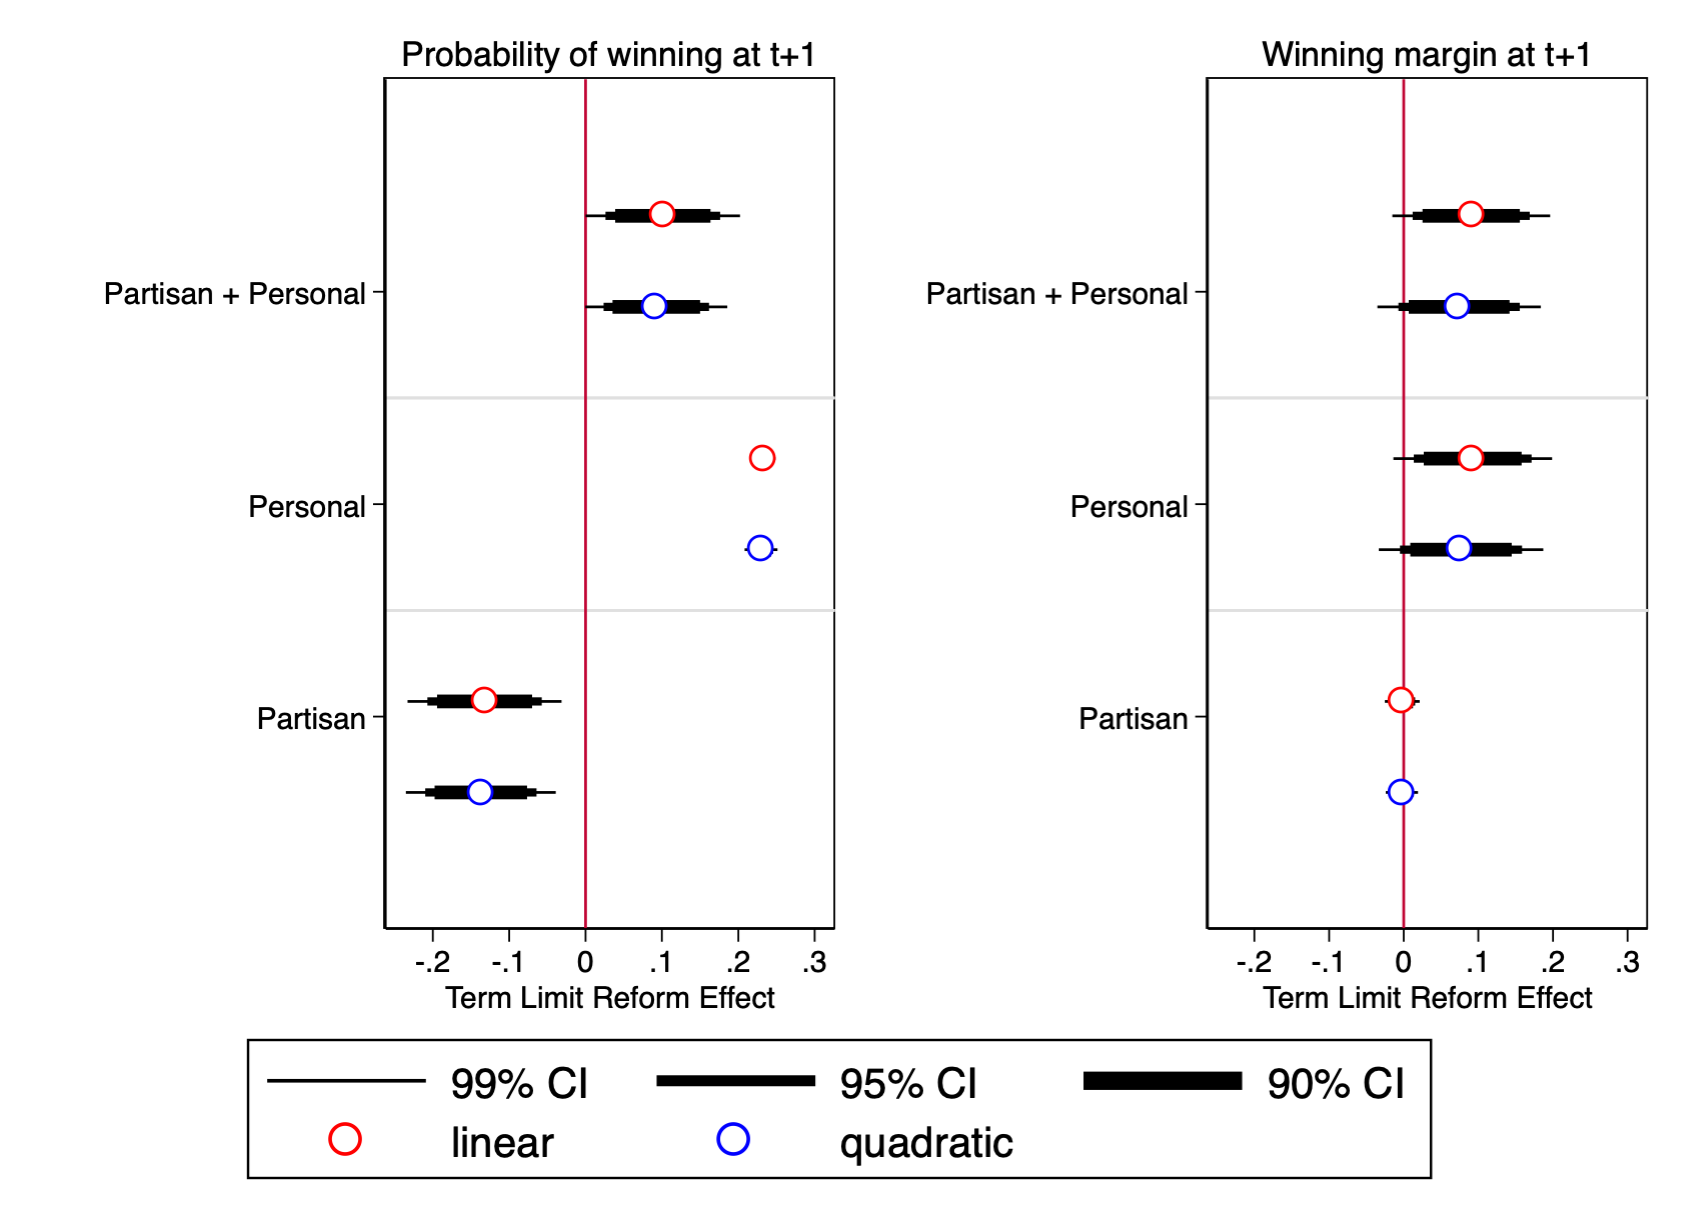
\includegraphics[width=0.9\textwidth]{../Figures_incumbency/twfe_personalvspartisan_advantage.png}
 
  \textbf{Note:} The left panel in figure \ref{fig:twfe_partisan&personal} shows the average treatment effect of the Term Limit Reform on the probability of winning in the following election using a difference in discontinuity of close elections design; the right panel shows the winning margin. Optimal bandwidths following \citet{calonicoetal_2014} are used. This analysis identifies the party that wins at $t-1$ and studies the effect of this party barely winning (or losing) at $t$ on outcomes at election $t+1$ following \citet{klasnja_titiunik_2017}.  
\end{figure} 
\end{comment}

\begin{figure}[h]   
\centering    
 \caption{Effect of Term Limit Reform on Partisan and Personal Incumbency Advantage, using winning margin in the next election \\ -difference-in-discontinuity of close elections design-}
 \label{fig:personal_vs_partisan_margin}
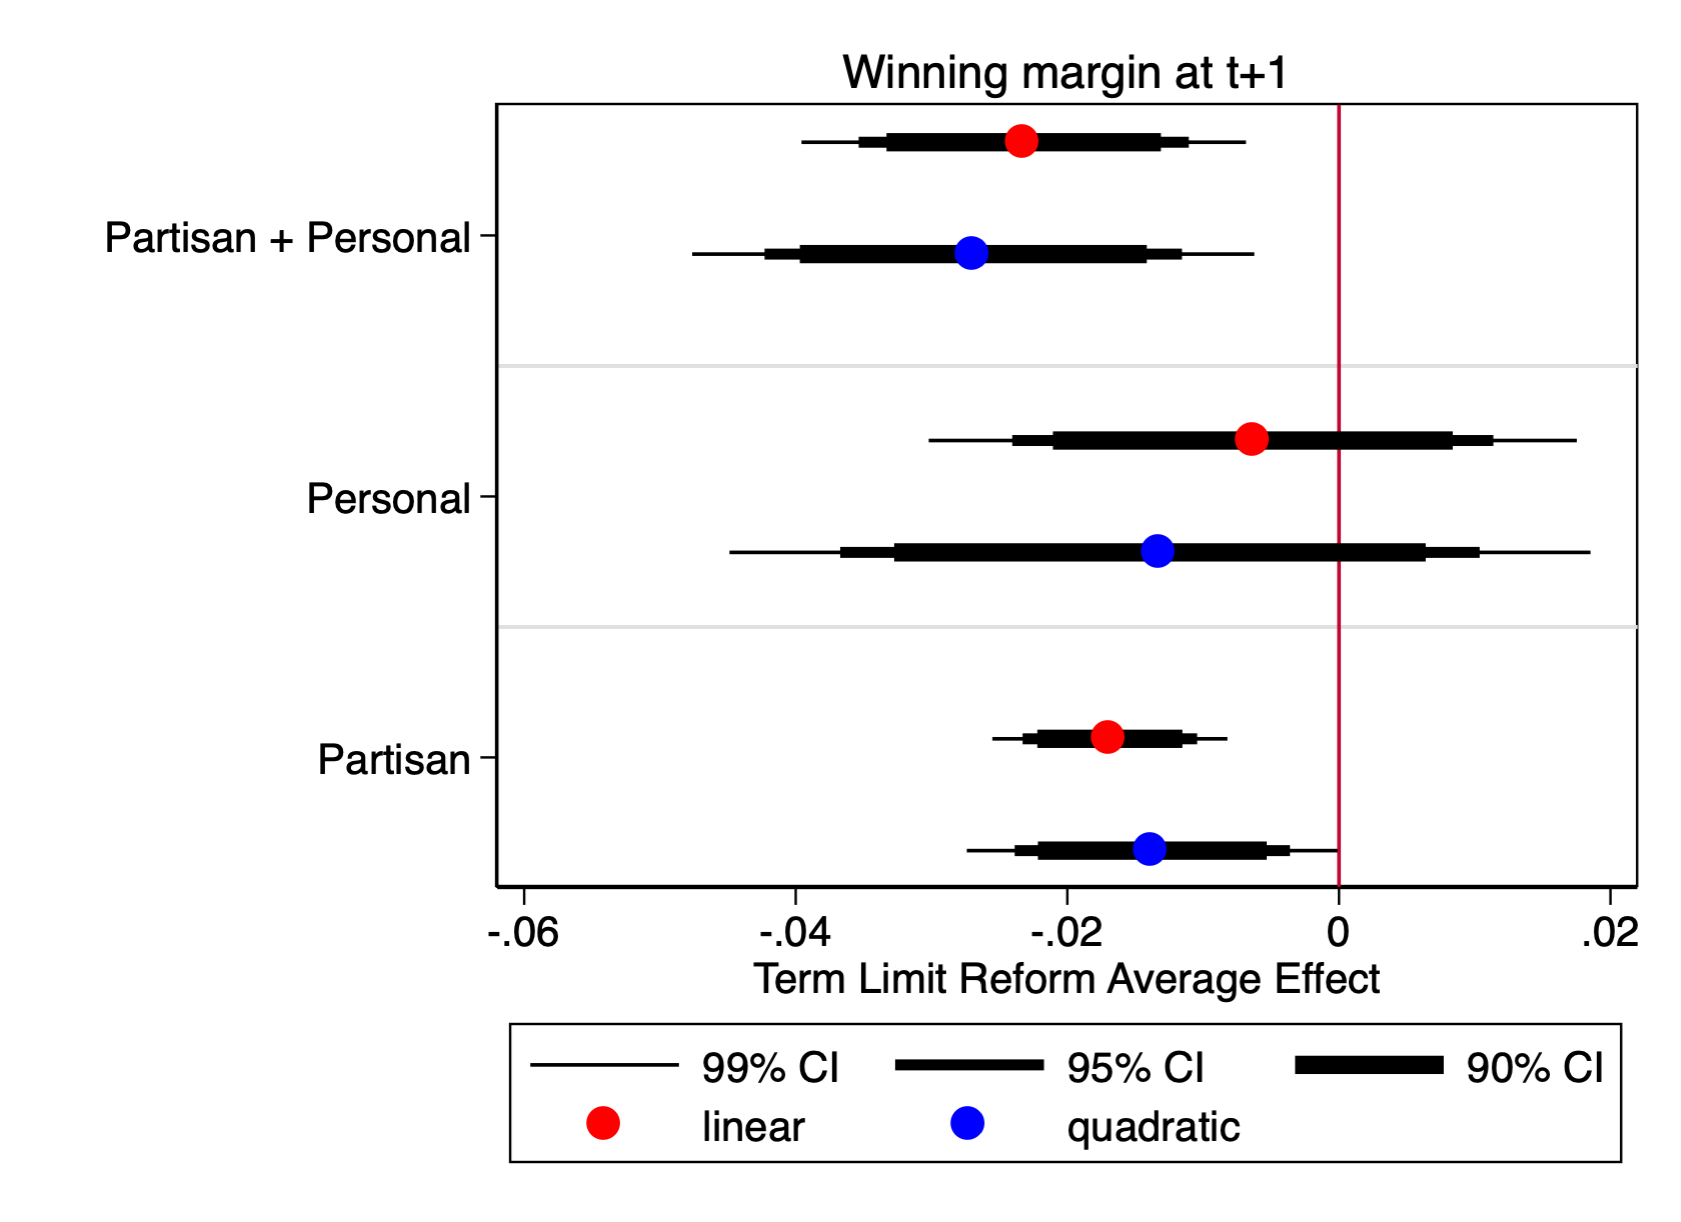
\includegraphics[width=0.9\textwidth]{../Figures_incumbency/partisan_personal_inc_advantage_margin.png}
       \captionsetup{justification=centering}
         
 \textbf{Note:} Figure \ref{fig:personal_vs_partisan_margin} shows the average treatment effect of the Term Limit Reform on the winning margin in the following election using a difference in discontinuity of close elections design. This average effect was estimated using the IW estimators following \citet{abraham_sun_2020} for each lead and lag relative to the first year a municipality implemented reelection. Optimal bandwidths following \citet{calonicoetal_2014} are used. Red and blue points show that parallel trends hold, while hollow ones imply pretrends. 
\end{figure}           

%Figure:
 \begin{figure}[h]   
\centering
 \caption{Personal and Partisan Incumbency Advantage, event study design}
 \label{fig:naive_partisan&personal}
 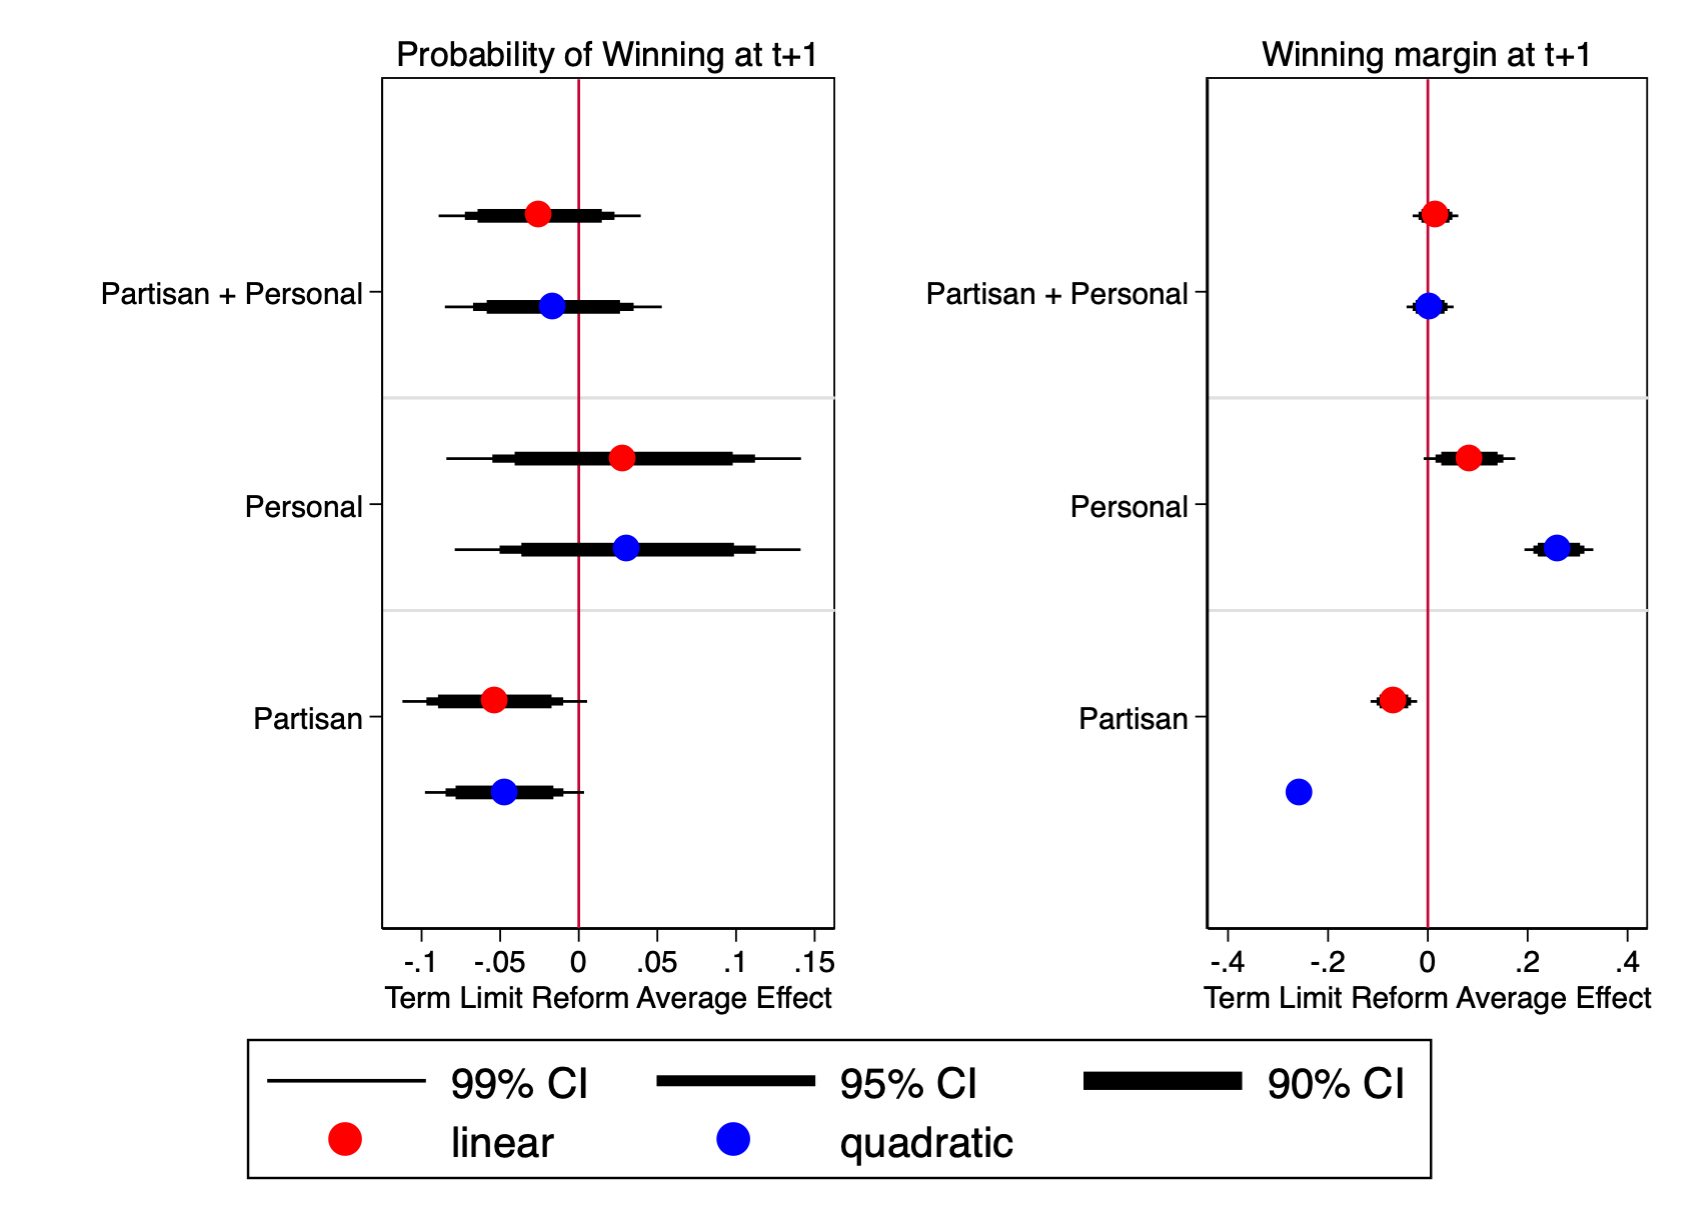
\includegraphics[width=0.9\textwidth]{../Figures_incumbency/naive_personalvspartisan_advantage.png}
 
  \textbf{Note:} The left panel in figure \ref{fig:naive_partisan&personal} shows the average treatment effect of the Term Limit Reform on the probability of winning in the following election using a difference in discontinuity of close elections design; the right panel shows the winning margin in the next election. Optimal bandwidths following \citet{calonicoetal_2014} are used. 
\end{figure} 
       



 \begin{figure}[h]   
\centering
 \caption{No discontinuous jump of covariates}
 \label{fig:jump_covariates}
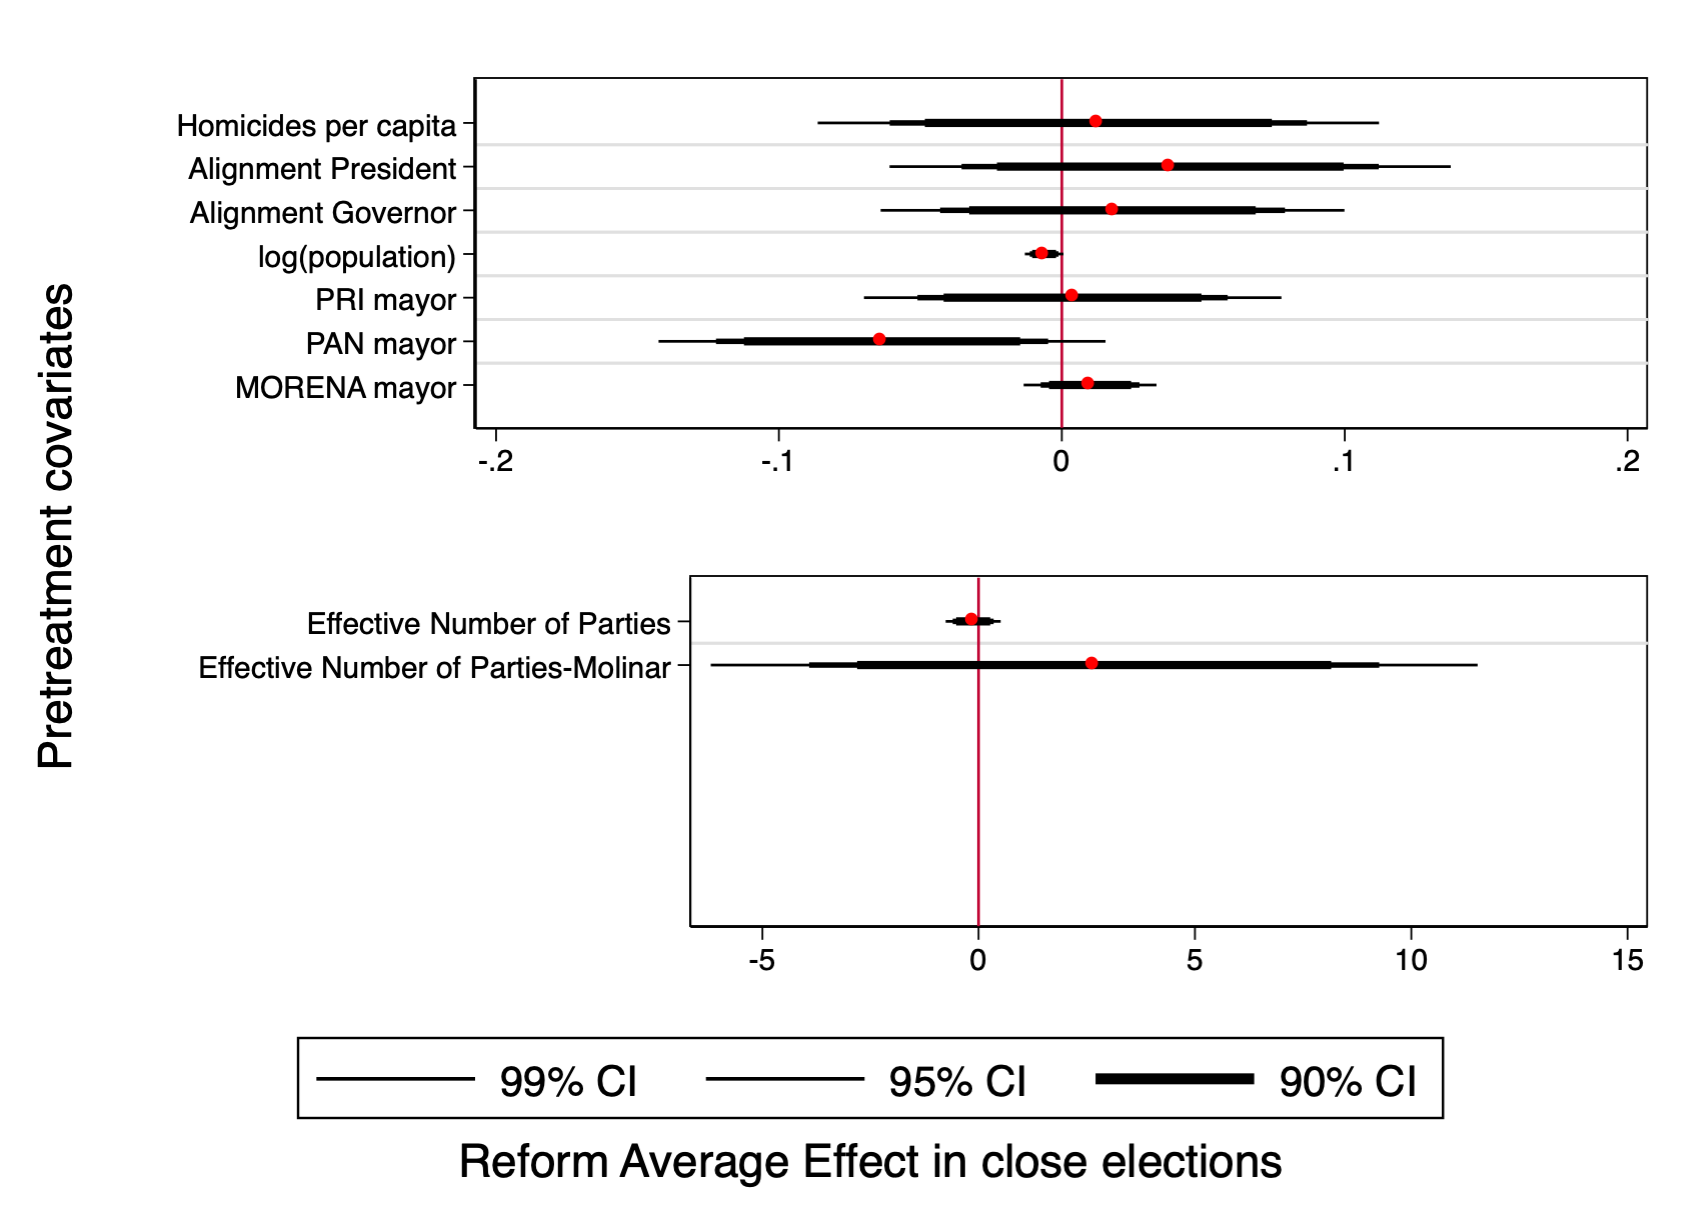
\includegraphics[width=0.9\textwidth]{../Figures_incumbency/nojump.png}
       \captionsetup{justification=centering}
    
 \textbf{Note:} Figure \ref{fig:jump_covariates} shows the average treatment effect of the Term Limit Reform on various pretreatment covariates using a difference in discontinuity of close elections design. This average effect was estimated using the IW estimators following \citet{abraham_sun_2020} for each lead and lag relative to the first year a municipality implemented reelection. Optimal bandwidths following \citet{calonicoetal_2014} are used. 
   
\end{figure} 


    
    
\begin{figure}[h]   
\centering
 \caption{McCrary Test}
 \label{fig:mccrary}
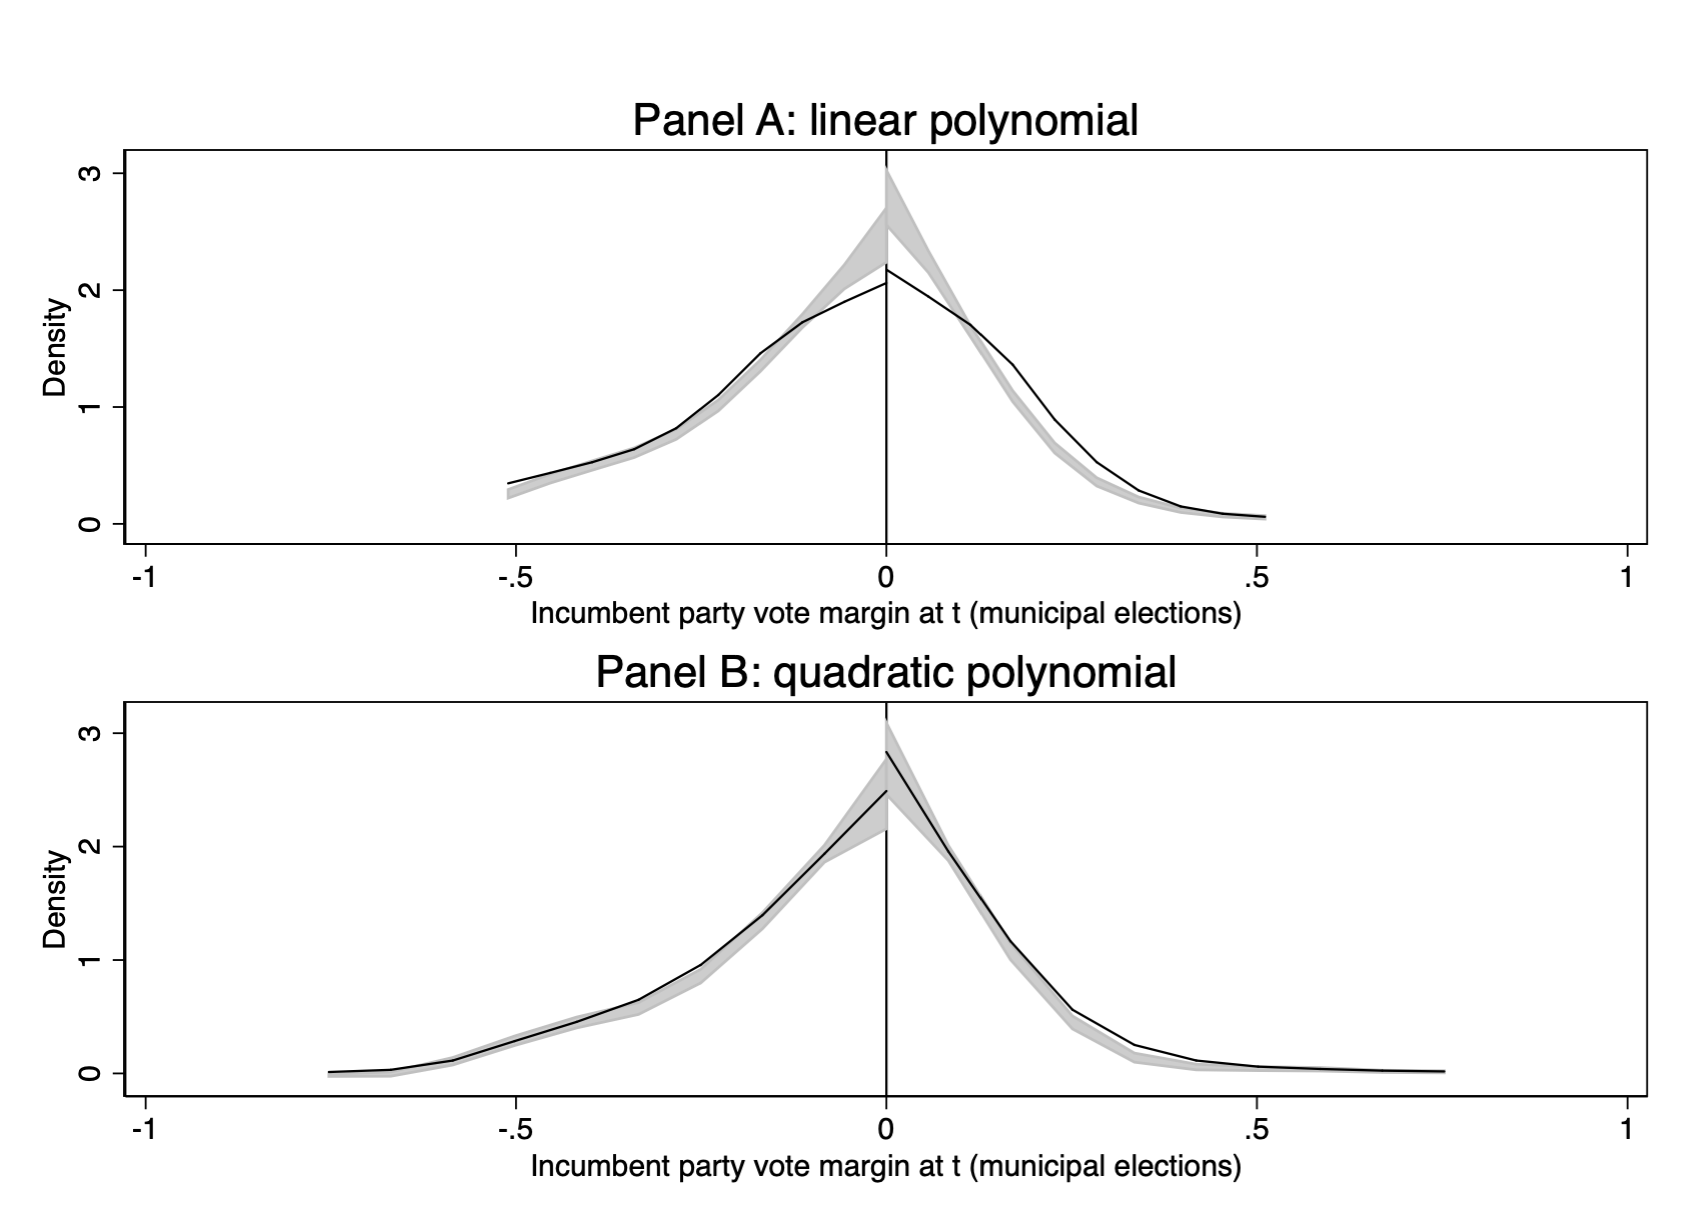
\includegraphics[width=1\textwidth]{../Figures_incumbency/mccrary_pol1_2.png}

       \captionsetup{justification=centering}
         
 \textbf{Note:} 95\% confidence intervals reported.
 
\end{figure} 


 \begin{figure}[h]   
\centering
 \caption{Testing Different Bandwidths}
 \label{fig:bandwidths}
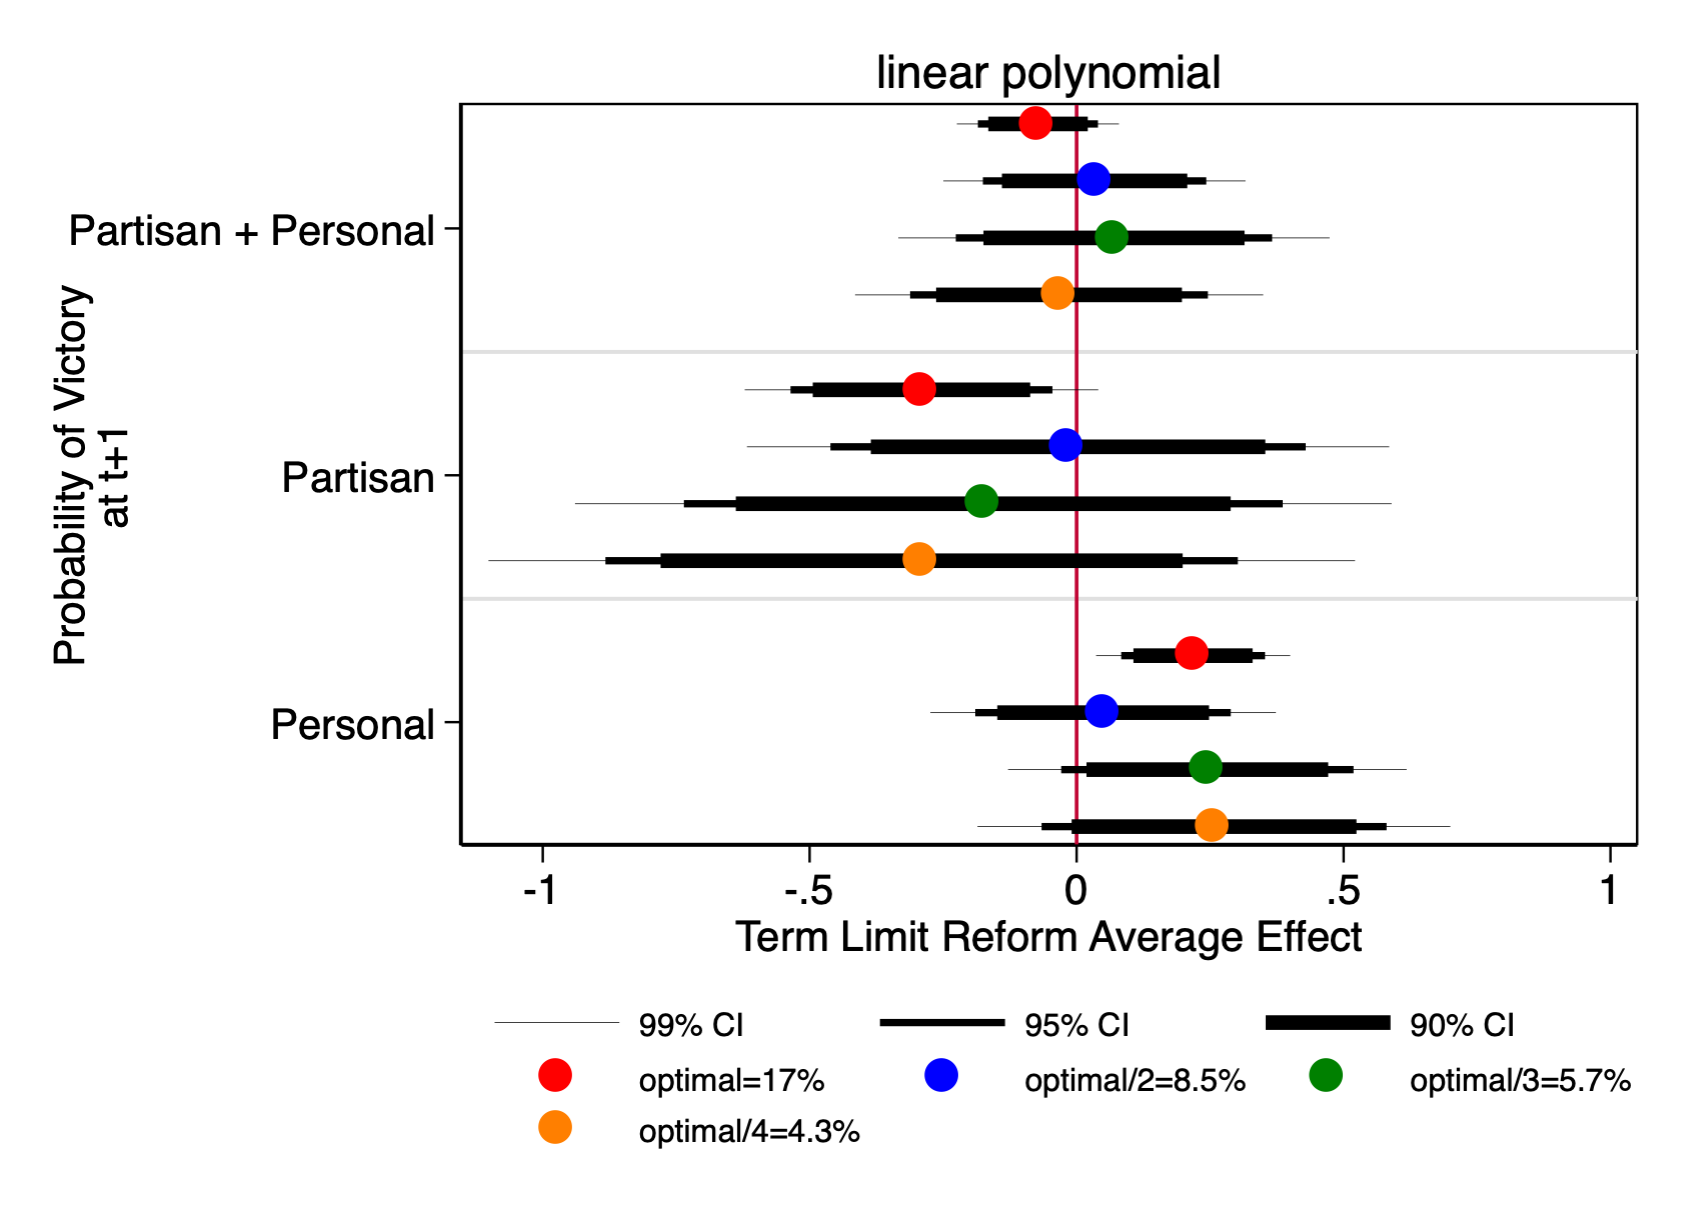
\includegraphics[width=0.65\textwidth]{../Figures_incumbency/many_bandwidths_linear.png}
       \captionsetup{justification=centering}
 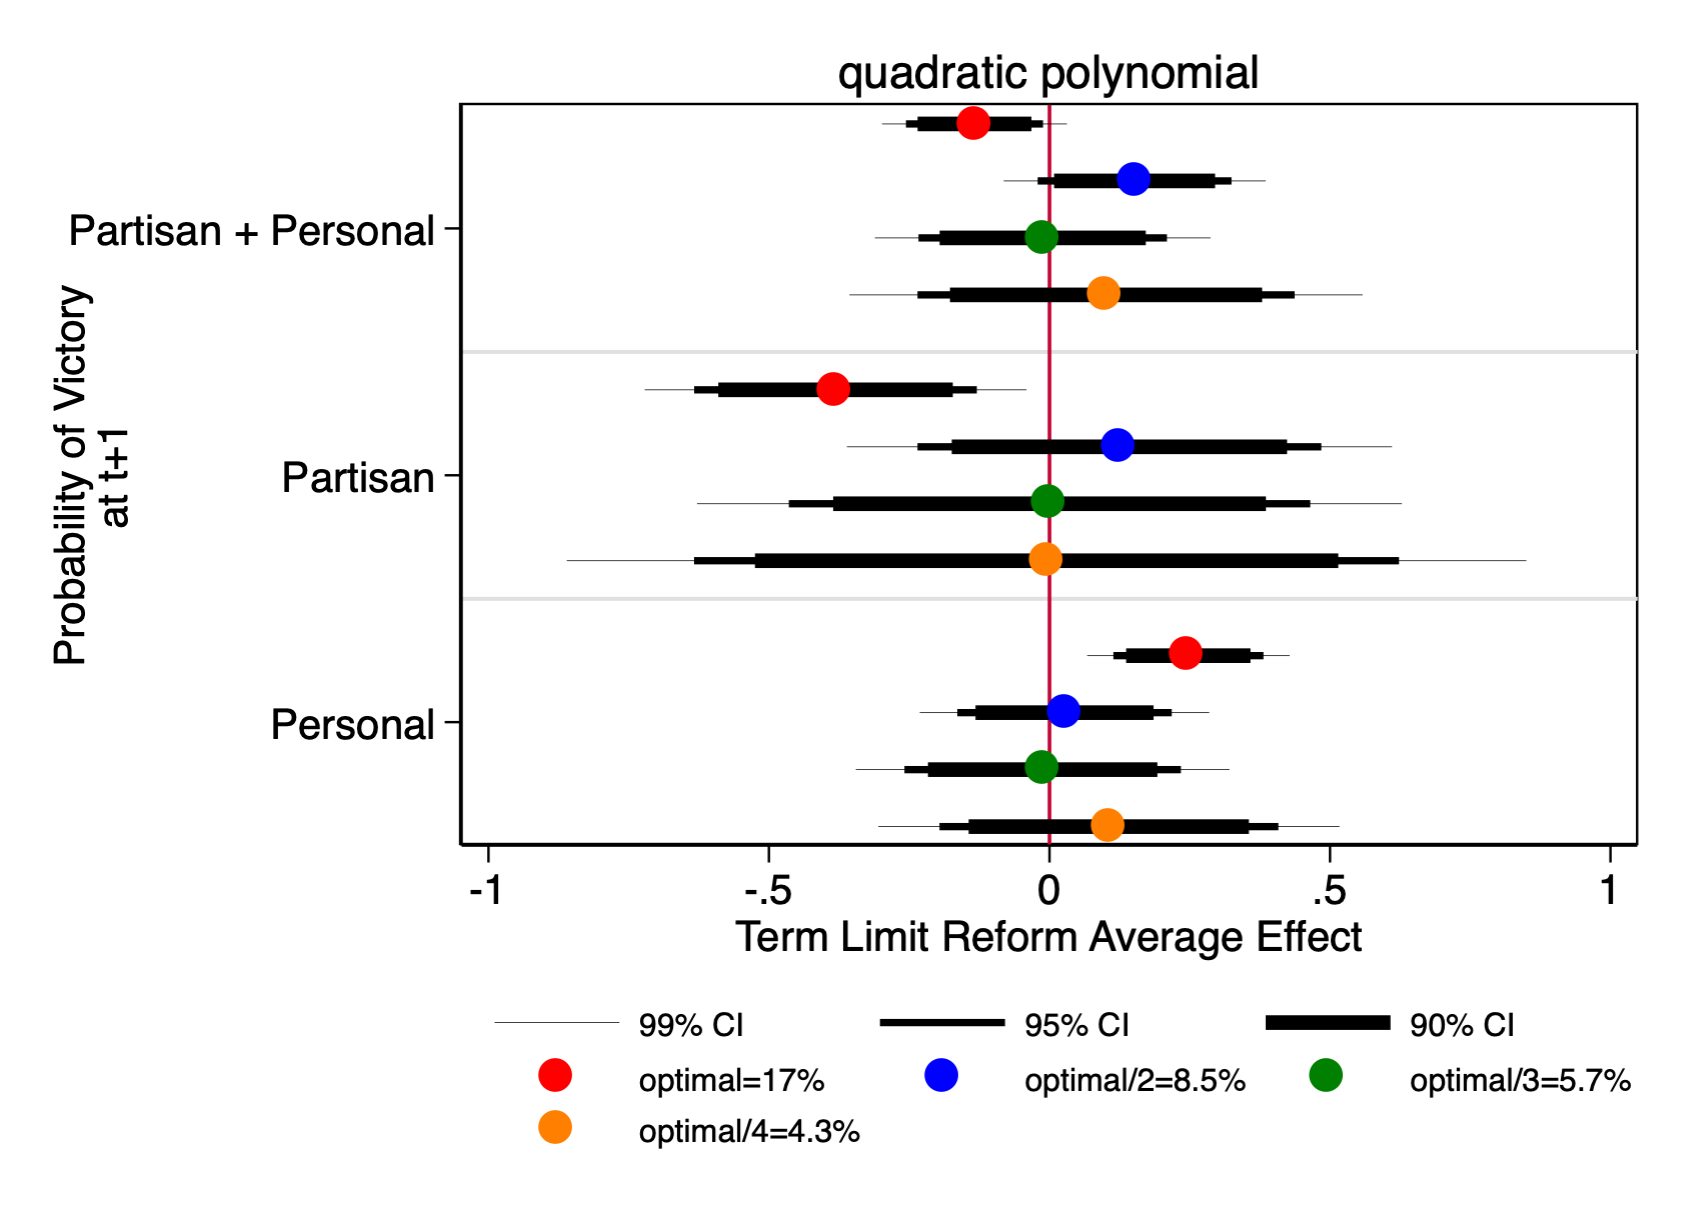
\includegraphics[width=0.65\textwidth]{../Figures_incumbency/many_bandwidths_quadratic.png}
  
 \textbf{Note:} Figure \ref{fig:bandwidths} shows the average treatment effect of the Term Limit Reform on the probability of victory in the next election. This average effect was estimated using the IW estimators following \citet{abraham_sun_2020} for each lead and lag relative to the first year a municipality implemented reelection. Various bandwidths are tested as well as the optimal bandwidths following \citet{calonicoetal_2014}. 
   
\end{figure}    


\begin{comment}
	
\begin{figure}[h]   
\centering
 \caption{Effect of Term Limit Reform on Fiscal Transfers, considering only municipalities with close elections}
 \label{fig:resources2}
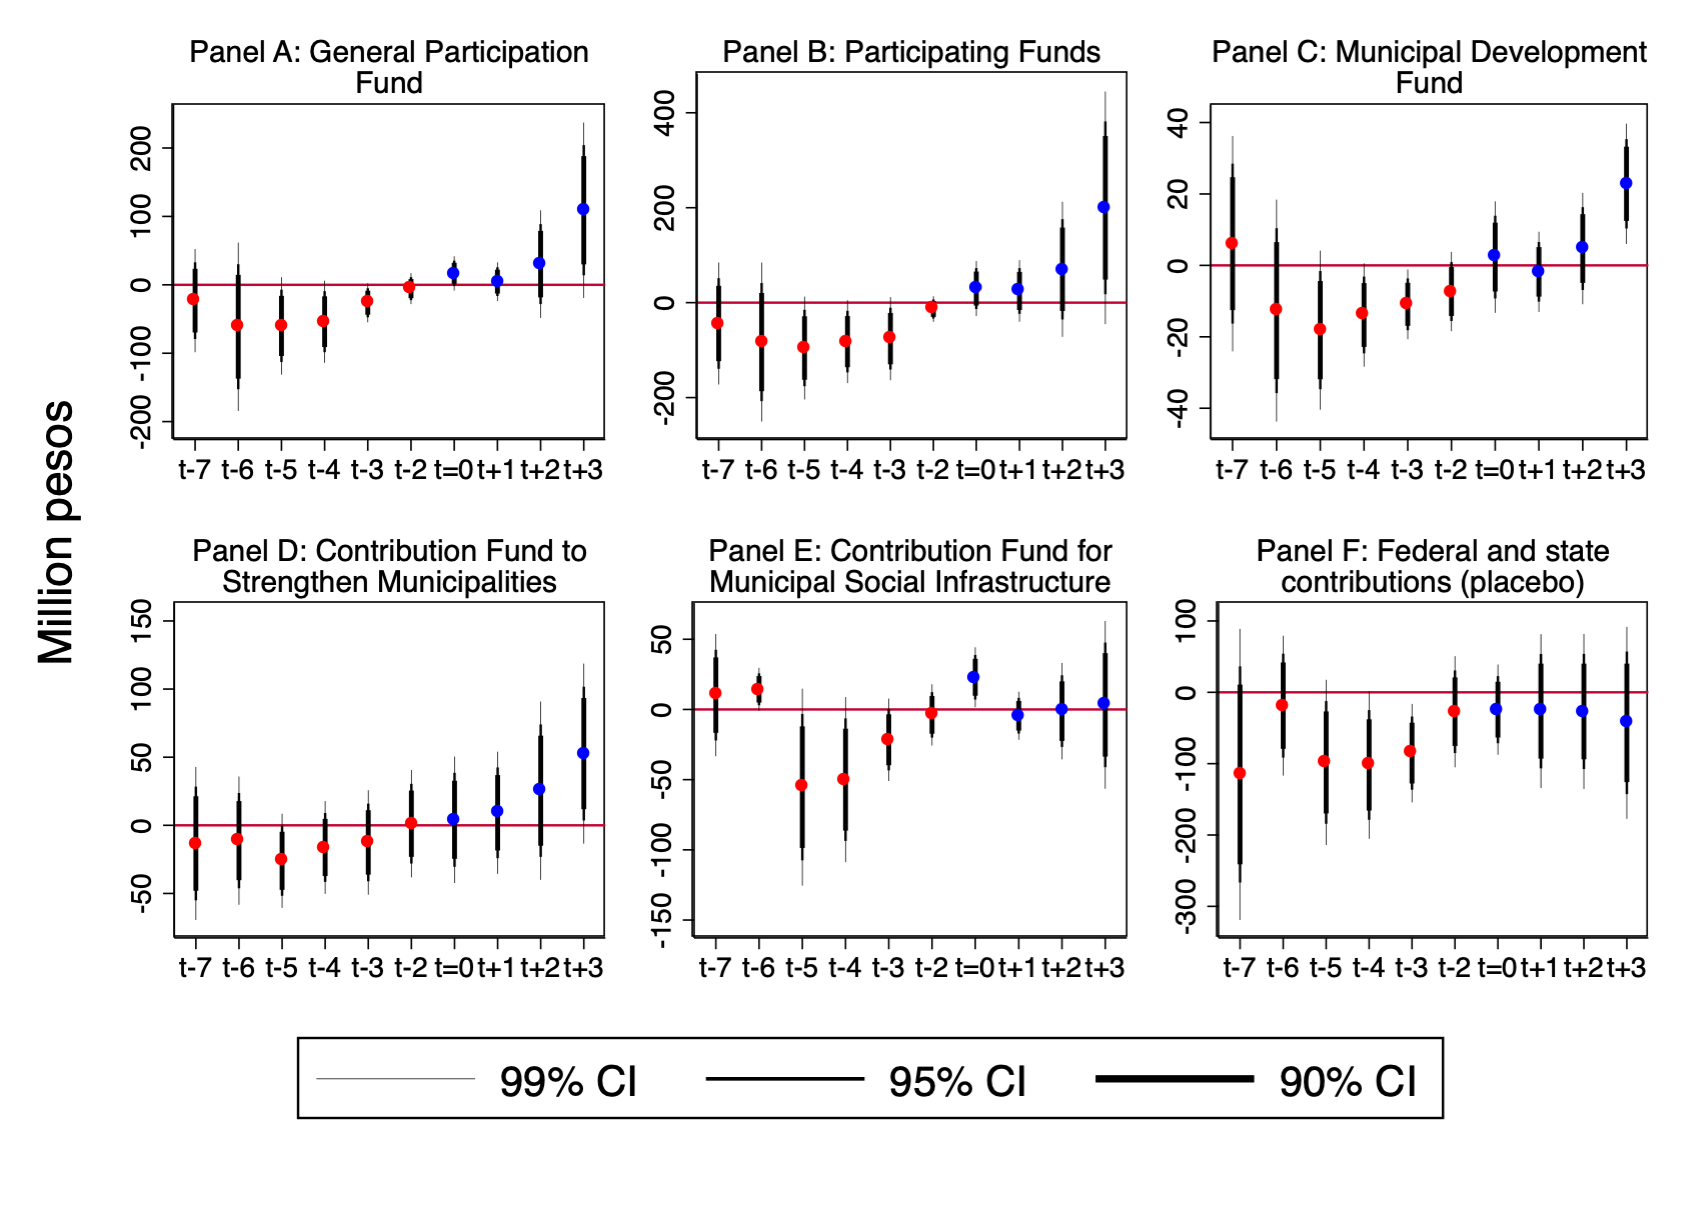
\includegraphics[width=0.9\textwidth]{../Figures_incumbency/resouce_based_incumbency_allyears.png}
       \captionsetup{justification=centering}
         
 \textbf{Note:} Figure \ref{fig:resources2} shows the average treatment effect of the Term Limit Reform on a dummy indicator of whether candidates hold a professional title. This average effect was estimated using the IW estimators following \citet{abraham_sun_2020} for each lead and lag relative to the first year a municipality implemented reelection. Same optimal bandwidths as those in Figure \ref{fig:parallel_trend} are used, as well as the same number of observations.  
       
\end{figure}  

 \end{comment}

\begin{comment}
	
 \begin{figure}[h]   
\centering
 \caption{Effect of Term Limit Reform on Municipal Expenses}
 \label{fig:expenses}
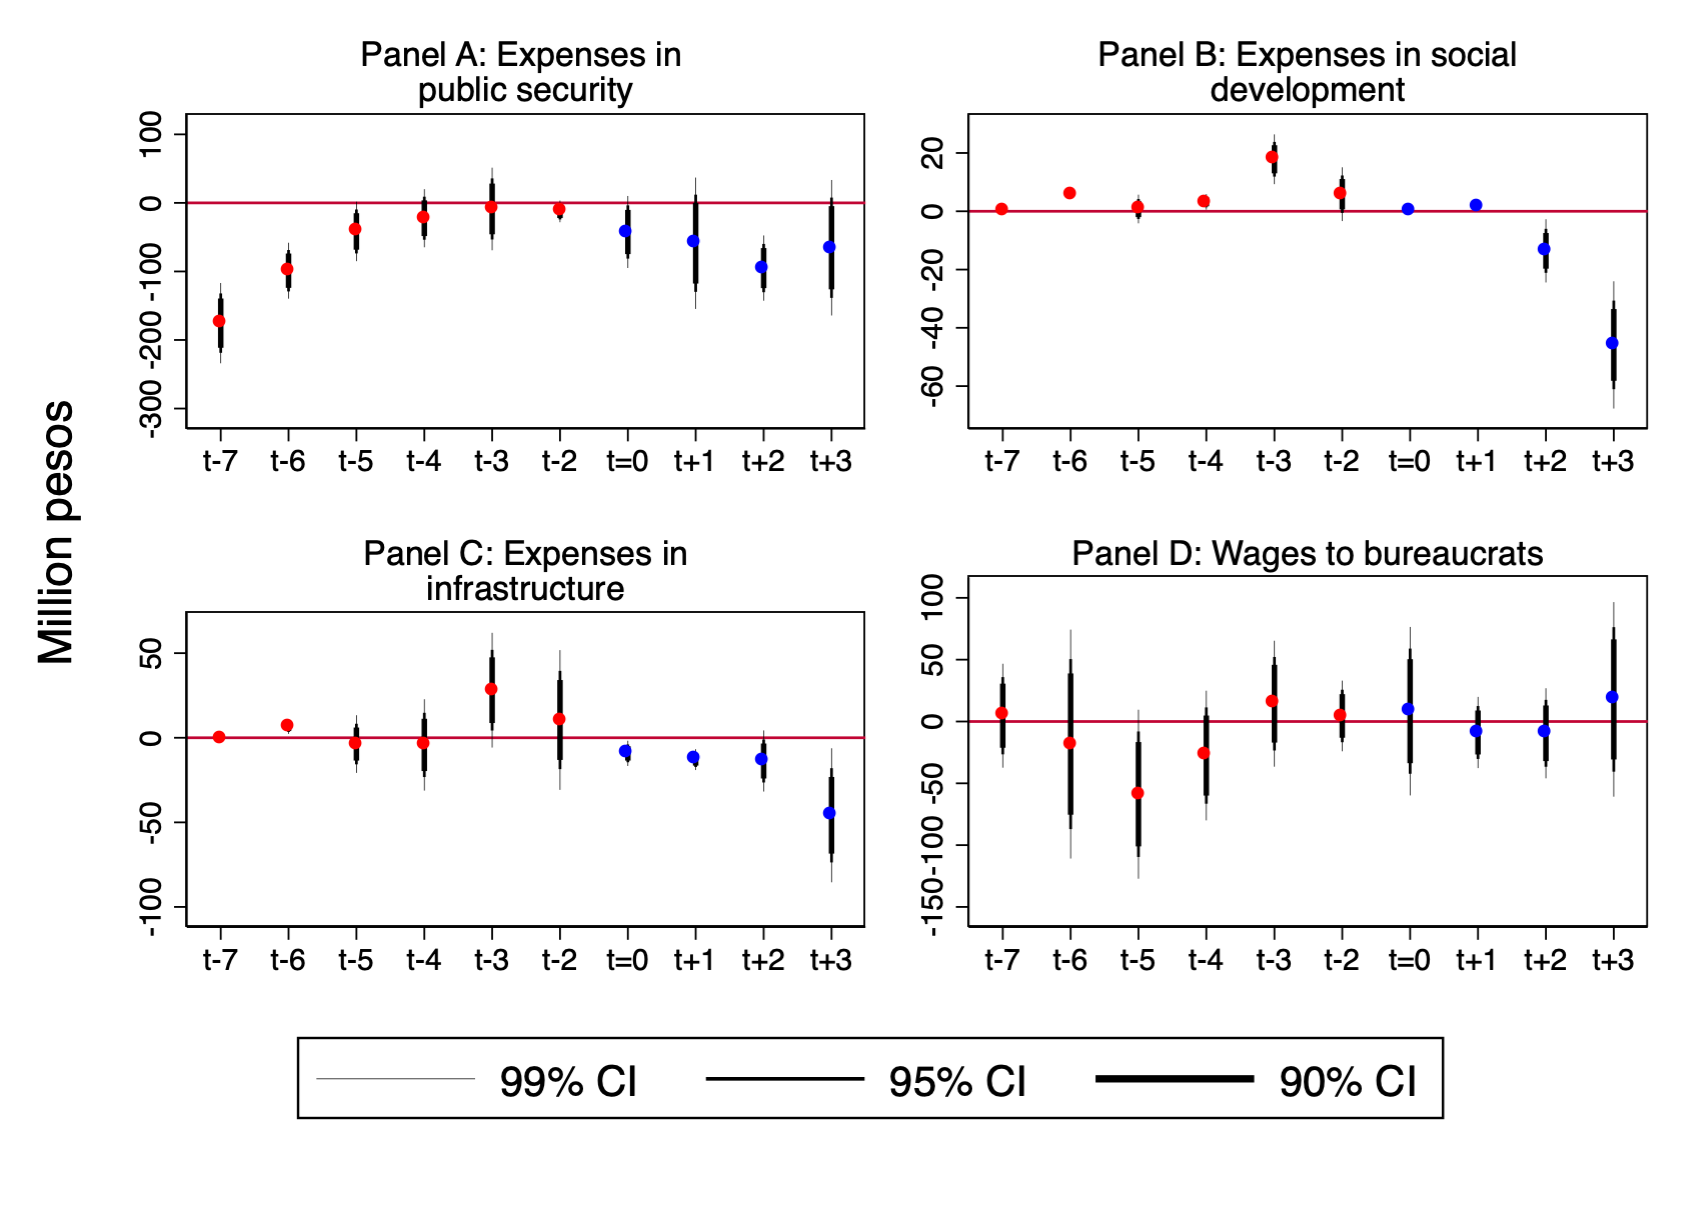
\includegraphics[width=0.9\textwidth]{../Figures/expenses_allyears.png}
       \captionsetup{justification=centering}
         
 \textbf{Note:} Figure \ref{fig:expenses} shows the average treatment effect of the Term Limit Reform on a dummy indicator of whether candidates hold a professional title. This average effect was estimated using the IW estimators following \citet{abraham_sun_2020} for each lead and lag relative to the first year a municipality implemented reelection. Same optimal bandwidths as those in Figure \ref{fig:main} are used, as well as the same number of observations.  
     
\end{figure}    
\end{comment}  

\clearpage
%%%%%%%%%%%%%%%%%%%%%%%%%%%%%%%%% 
%%%% RDD design

 \renewcommand{\thetable}{B-\arabic{table}}
\setcounter{table}{0}
 
\renewcommand{\thefigure}{B-\arabic{figure}}
\setcounter{figure}{0}

\section{Regression Discontinuity Design of close elections, comparing elections with and without term limits \label{appendix:rdd}} 

I begin by visualizing the effect of the reform on incumbency advantage.  Figure \ref{fig:incumbency_advantage} presents the RDD estimate of close elections on incumbency advantage  within an optimal bandwidth distance $h$ from the cutoff (0), and a quadratic polynomial:\footnote{A triangular kernel is used. Results are similar when using other polynomial functional forms.} Panel A shows a comparison of municipalities with incumbents at $t-1$ that barely won to those that barely lost in $t$ on the probability of electoral victory at $t+1$,\footnote{Incumbency advantage measure following \citet{klasnja_titiunik_2017}.} taking into account all elections from 1979 to 2014 (i.e. prior to the term-limit reform); Panel B shows the same comparison but restricting the sample to municipalities that implemented reelection after 2014. I do not consider those municipal elections that after 2014 did not implement reelection. Table \ref{tab:rdd} shows RD estimates using multiple polynomial functional forms. Even though RD estimates are biased in this setting, especially for Panel B in Figure \ref{fig:incumbency_advantage} (and even columns in Table \ref{tab:rdd}) since in the presence of staggered treatment timing and heterogeneous treatment effects across cohorts are not causally interpretable since we are considering both early vs late adopters of the reform on the treated,\footnote{The next iteration of this working paper will show this proof in the Appendix for RD designs.} they provide a striking depiction of what occurred before and after the electoral reform. 


\begin{figure}[H]
\centering
\caption{Effect of Term Limit Reform on Incumbency Advantage, quadratic polynomial}
  \label{fig:incumbency_advantage} 

	{\textbf Figure A: Probability of winning at t+1}
	 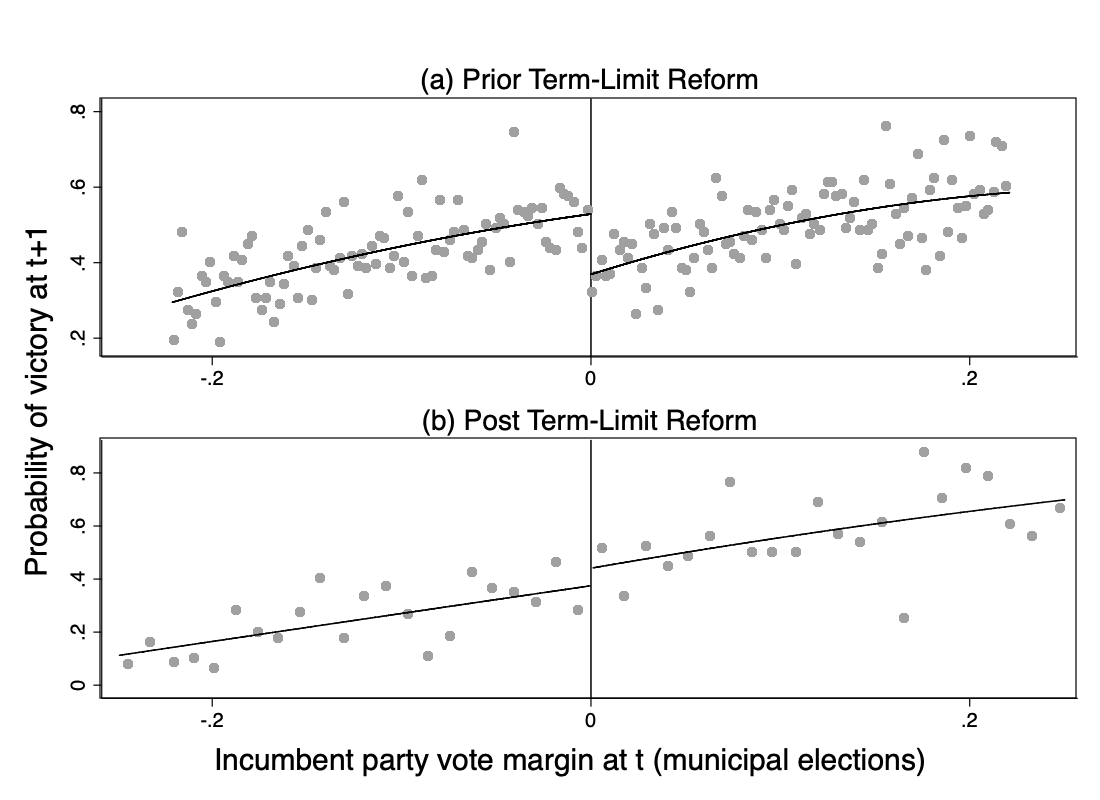
\includegraphics[width=0.6\textwidth]{../Figures_incumbency/RDD_incumbency_pol2.png}
	 \\
	{\textbf Figure B: Winning margin at t+1}

 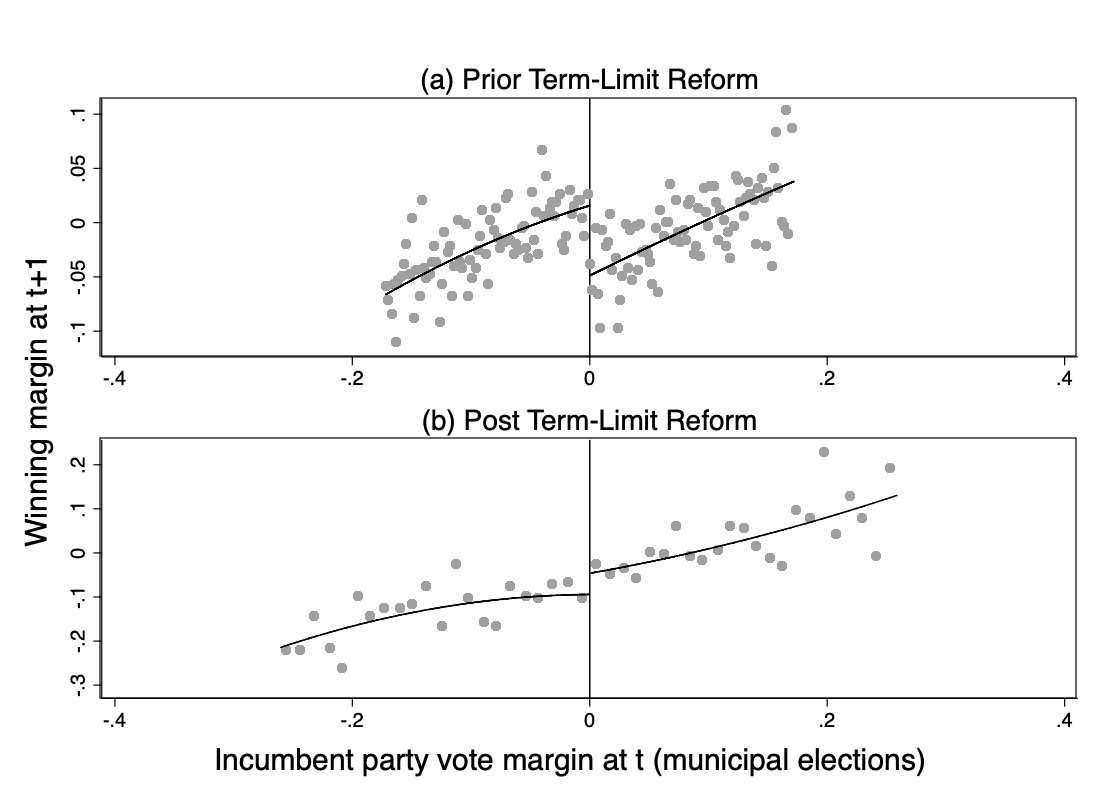
\includegraphics[width=0.6\textwidth]{../Figures_incumbency/RDD_incumbency_margin_pol2.png}
     \captionsetup{justification=centering}  
       
\end{figure} 
       Note: Regression Discontinuity design of close elections on incumbency advantage. Panel (a) considers all elections from 1979 to 2014. Panel (b) considers all elections after 2014 for municipalities that implemented reelection.) 
\\
       
Before the reform, there was a negative statistical significant difference between municipalities that barely won and lost on the probability of success in the next election. This incumbency \emph{disadvantage} aligns strongly with a similar result found by \citet{klasnja_titiunik_2017} for the case of Mexico. \citet{klasnja_titiunik_2017} find that an incumbent party that is barely reelected suffers a reduction in the probability of winning the following election of 28 percentage points. In contrast, I find a reduction between 10.7 to 11.32 percentage points, a finding that considers 20 more years of elections since \citet{klasnja_titiunik_2017} cap their data from 1997 to 2009, while I consider elections since 1979 to 2014. 

More interesting is the finding that after reelection takes place the previous incumbency disadvantage disappears as noted by a positive and non-statistical significant difference between municipalities that barely lost and won an election. This initial RDD results provide suggestive evidence that the electoral reform generated an increase in the probability of victory in the next election for municipalities that barely won an election relative to those that barely lost. These estimates, however, may be biased. By comparing term limit and non-term limit elections we are assuming there are parallel trends for identification which might not be the case. Furthermore, as \citet{eggers_2017} even when comparing close elections, a potential difference in the quality of incumbents and challengers may exist. 
 
 \\ 
  
%Table:
\begin{table}[!htbp]\def\sym#1{\ifmmode^{#1}\else\(^{#1}\)\fi}
\caption{Regression Discontinuity Design of Close Elections on Incumbency Advantage: Comparison of term and non-term limited elections}
\label{tab:rdd}
\begin{center} 
\scalebox{1}{
\begin{tabular}{lcccc}
 
\hline \hline   
\\       
   
\multicolumn{5}{l}{Dependent variable:}\\
  
\\
            &\multicolumn{2}{c}{linear polynomial}      &\multicolumn{2}{c}{quadratic polynomial}   \\\cmidrule(lr){2-3}\cmidrule(lr){4-5}
            &\multicolumn{1}{c}{(1)}         &\multicolumn{1}{c}{(2)}         &\multicolumn{1}{c}{(3)}         &\multicolumn{1}{c}{(4)}         \\
\addlinespace
Probability of victory at t+1&      0.0711         &     -0.1589\sym{***}&      0.0554         &     -0.1616\sym{***}\\
            &    (0.0636)         &    (0.0260)         &    (0.0846)         &    (0.0323)         \\
\addlinespace
Observations&         887         &       6,072         &         954         &       7,287         \\
Term Limit  &                     &  \checkmark         &                     &  \checkmark         \\
 
\\
            &\multicolumn{2}{c}{linear polynomial}      &\multicolumn{2}{c}{quadratic polynomial}   \\\cmidrule(lr){2-3}\cmidrule(lr){4-5}
            &\multicolumn{1}{c}{(1)}         &\multicolumn{1}{c}{(2)}         &\multicolumn{1}{c}{(3)}         &\multicolumn{1}{c}{(4)}         \\
\addlinespace
Winning margin at t+1&      0.0307         &     -0.0452\sym{***}&      0.0390         &     -0.0463\sym{***}\\
            &    (0.0305)         &    (0.0081)         &    (0.0343)         &    (0.0102)         \\
\addlinespace
Observations&         677         &       7,328         &         955         &       9,157         \\
Term Limit  &                     &  \checkmark         &                     &  \checkmark         \\
 
 
                 
\hline \hline   
\multicolumn{5}{p{0.8\textwidth}}{\footnotesize{Notes: Standard errors in parentheses, with the following significance-level: $^{***}$ 1\%; $^{**}$ 5\%; and $^*$ 10\%, that refer to two-sided t-test. Optimal bandwidth following \citet{calonicoetal_2014} $^a$ Incumbency advantage measured following \citet{klasnja_titiunik_2017}. 
  }} \\  
\end{tabular}         
}
\end{center} 
\end{table} 

\clearpage
  
\end{document}
